\documentclass[aspectratio=169,10pt]{beamer}

\usepackage{lmodern}
\usepackage[utf8]{inputenc}
\usepackage[T1]{fontenc}
\usepackage[english]{babel}
\usepackage{amsmath,amssymb,amsfonts}
\usepackage{booktabs}
\usepackage{colortbl}
\usepackage{graphicx}
\usepackage{xcolor}
\usepackage{fontawesome5}
\usepackage{listings}
\usepackage{etoolbox}
\usepackage{tikz}
\usetikzlibrary{positioning, arrows.meta}

\usetikzlibrary{shapes.symbols,shapes.geometric,arrows.meta,positioning,fit,calc,shadows,decorations.pathreplacing,decorations.pathmorphing,shapes.gates.logic.US}

\usetheme{Madrid}
\useinnertheme{rounded}
\useoutertheme{miniframes}

\definecolor{DeepBlue}{HTML}{283593}% template indigo (colour rules v6)
\definecolor{AccentOrange}{RGB}{235,90,20}
\definecolor{LightGray}{RGB}{245,246,250}
\definecolor{mygreen}{RGB}{0,153,37}
\definecolor{VSDarkBg}{RGB}{25,25,25}
\definecolor{VSText}{RGB}{245,245,245}
\definecolor{VSBlue}{RGB}{80,180,255}
\definecolor{VSPurple}{RGB}{210,110,210}
\definecolor{VSString}{RGB}{255,140,80}
\definecolor{VSComment}{RGB}{80,220,80}
\definecolor{MacRed}{RGB}{255,95,86}
\definecolor{MacYellow}{RGB}{255,189,46}
\definecolor{MacGreen}{RGB}{39,201,63}
\definecolor{ProgramPurple}{RGB}{124,58,180}
\definecolor{StorageBlue}{RGB}{30,120,200}

% ---------- course palette (colour rules v6) ----------
% actors and categories: fills only
\definecolor{sIndigo}{HTML}{5C6BC0}
\definecolor{sPink}{HTML}{EC407A}
\definecolor{sViolet}{HTML}{7E57C2}
\definecolor{sAmber}{HTML}{FFB300}   % black text on it
\definecolor{sTeal}{HTML}{26A69A}
\definecolor{sBrown}{HTML}{8D6E63}
% text variants that stay readable on white
\definecolor{sPinkText}{HTML}{C2185B}
\definecolor{sAmberText}{HTML}{A06A00}
\definecolor{sTealText}{HTML}{00796B}
% actions: frames only (executes, read, write); results: signs only
\definecolor{aExec}{HTML}{43A047}
\definecolor{aRead}{HTML}{1E88E5}
\definecolor{aWrite}{HTML}{E53935}
% neutral (Blue Grey): hardware, data, waveforms
\definecolor{nInk}{HTML}{37474F}
\definecolor{nLine}{HTML}{90A4AE}
\definecolor{nLight}{HTML}{CFD8DC}
\definecolor{nFill}{HTML}{ECEFF1}
\definecolor{nIdle}{HTML}{E0E0E0}
\tikzset{
  aexec/.style={draw=aExec, line width=1.6pt},
  aread/.style={draw=aRead, line width=1.6pt, dash pattern=on 3pt off 2pt},
  awrite/.style={draw=aWrite, line width=2.4pt},
}
\newcommand{\ok}{\textcolor{aExec}{\faCheck}}
\newcommand{\nok}{\textcolor{aWrite}{\faTimes}}


\setbeamercolor{palette primary}{bg=DeepBlue,fg=white}
\setbeamercolor{palette secondary}{bg=DeepBlue!80!black,fg=white}
\setbeamercolor{palette tertiary}{bg=DeepBlue!90!black,fg=white}
\setbeamercolor{title}{bg=DeepBlue,fg=white}
\setbeamercolor{frametitle}{bg=DeepBlue,fg=white}
\setbeamercolor{structure}{fg=DeepBlue}
\setbeamercolor{item}{fg=AccentOrange}
\setbeamercolor{alerted text}{fg=AccentOrange}
\setbeamercolor{block title}{bg=DeepBlue,fg=white}
\setbeamercolor{block body}{bg=LightGray,fg=black}
\setbeamercolor{block title example}{bg=AccentOrange,fg=white}
\setbeamercolor{block body example}{bg=AccentOrange!10,fg=black}
\setbeamercolor{vscodelisting}{bg=VSDarkBg}
\setbeamertemplate{blocks}[rounded][shadow=true]
\setbeamertemplate{navigation symbols}{}
\setbeamertemplate{itemize items}[circle]
\setbeamertemplate{enumerate items}[default]
\setbeamercolor{enumerate item}{fg=DeepBlue}
\setbeamerfont{enumerate item}{series=\bfseries}

% ---------- helpers used by the von Neumann section ----------
\tikzset{
  memcell/.style={draw=nLine, minimum width=2.6cm, minimum height=0.45cm,
    inner sep=1pt, font=\ttfamily\scriptsize, align=center},
  instrcell/.style={memcell, fill=sViolet!18},
  datacell/.style={memcell, fill=sPink!18},
  addr/.style={font=\ttfamily\scriptsize, text=nInk},
}
% numbered orange badge for assumptions
\newcommand{\num}[1]{\tikz[baseline=(n.base)]\node[circle,fill=AccentOrange,text=white,
  inner sep=1.6pt,font=\bfseries\scriptsize] (n) {#1};}
% mini memory stack with the program counter pointing at cell #2
% #1 = x offset, #2 = highlighted cell (0-3), #3 = text of cell 3, #4 = panel heading
\newcommand{\pcstack}[4]{%
  \node[font=\scriptsize\bfseries, text=nInk] at (#1,0.55) {#4};
  \foreach \i/\t in {0/{LOAD 6},1/{ADD 7},2/{STORE 8},3/{#3}} {
    \ifnum\i=#2
      \node[instrcell, minimum width=1.7cm, aexec] at (#1,{-0.45*\i}) {\t};
    \else
      \node[instrcell, minimum width=1.7cm] at (#1,{-0.45*\i}) {\t};
    \fi
    \node[addr, anchor=west] at ({#1+0.92},{-0.45*\i}) {\i};
  }
  \node[anchor=east, text=AccentOrange, font=\scriptsize\bfseries] at ({#1-0.92},{-0.45*#2}) {PC $\rightarrow$};
}

% ---------- helpers for the dilemma / decision slides ----------
% option card: #1 title, #2 small diagram, #3 advantage, #4 drawback
% (all cards use the same neutral style so the colour does not reveal the answer)
\newcommand{\optcard}[4]{%
  \begin{beamercolorbox}[rounded=true,sep=0.16cm,wd=\linewidth]{block body}
    \centering\small\textbf{#1}\\[0.1cm]
    #2\\[0.1cm]
    \raggedright\footnotesize
    \textcolor{aExec}{\textbf{+}}\ #3\\[0.06cm]
    \textcolor{aWrite}{\textbf{$-$}}\ #4
  \end{beamercolorbox}}

% progress strip: #1 = number of decisions already made
\newcommand{\progress}[1]{%
  {\centering
  \begin{tikzpicture}
    \foreach \i/\t in {1/Stored program,2/Shared memory,3/Binary,4/Sequential,5/Separate units} {
      \ifnum\i>#1
        \node[draw=nLine, dashed, rounded corners=3pt, text=nLine, font=\tiny\bfseries,
          minimum width=2.45cm, minimum height=0.36cm, inner sep=1pt] at ({(\i-3)*2.6},0) {\i\ \t};
      \else
        \node[draw=DeepBlue, fill=DeepBlue, rounded corners=3pt, text=white, font=\tiny\bfseries,
          minimum width=2.45cm, minimum height=0.36cm, inner sep=1pt] at ({(\i-3)*2.6},0) {\i\ \t};
      \fi
    }
  \end{tikzpicture}\par}}

% ----- small diagrams used on the dilemma slides -----
\tikzset{smallcell/.style={draw=nLine, minimum height=0.27cm, inner sep=0.5pt,
  font=\ttfamily\tiny, align=center}}

\newcommand{\diagWired}{\begin{tikzpicture}
  \node[draw=AccentOrange, very thick, rounded corners=4pt, fill=AccentOrange!12, minimum width=2.5cm,
    minimum height=0.85cm, font=\scriptsize, align=center]
    {\textcolor{AccentOrange}{\faWrench}\ fixed circuit\\[-1pt]program = wiring};
\end{tikzpicture}}

\newcommand{\diagTape}{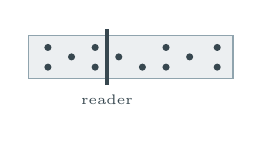
\begin{tikzpicture}
  \draw[draw=nLine, fill=nFill] (0,0) rectangle (2.6,0.55);
  \foreach \x/\y in {0.25/0.15,0.25/0.4,0.55/0.28,0.85/0.15,0.85/0.4,1.15/0.28,1.45/0.15,1.75/0.4,1.75/0.15,2.05/0.28,2.4/0.15,2.4/0.4}
    {\fill[nInk] (\x,\y) circle (0.045);}
  \draw[nInk, very thick] (1.0,-0.08) -- (1.0,0.63);
  \node[font=\tiny, text=nInk, anchor=north] at (1.0,-0.08) {reader};
\end{tikzpicture}}

\newcommand{\diagMemStackSmall}{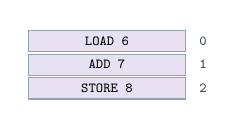
\begin{tikzpicture}
  \node[smallcell, fill=sViolet!18, minimum width=2.0cm] at (0,0.3) {LOAD 6};
  \node[smallcell, fill=sViolet!18, minimum width=2.0cm] at (0,0) {ADD 7};
  \node[smallcell, fill=sViolet!18, minimum width=2.0cm] at (0,-0.3) {STORE 8};
  \node[addr, font=\ttfamily\tiny, anchor=west] at (1.05,0.3) {0};
  \node[addr, font=\ttfamily\tiny, anchor=west] at (1.05,0) {1};
  \node[addr, font=\ttfamily\tiny, anchor=west] at (1.05,-0.3) {2};
\end{tikzpicture}}

\newcommand{\diagTwoMem}{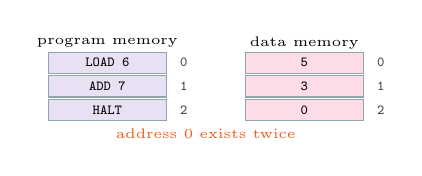
\begin{tikzpicture}
  \node[font=\tiny] at (0,0.55) {program memory};
  \node[font=\tiny] at (2.5,0.55) {data memory};
  \node[smallcell, fill=sViolet!18, minimum width=1.5cm] at (0,0.3) {LOAD 6};
  \node[smallcell, fill=sViolet!18, minimum width=1.5cm] at (0,0) {ADD 7};
  \node[smallcell, fill=sViolet!18, minimum width=1.5cm] at (0,-0.3) {HALT};
  \node[smallcell, fill=sPink!18, minimum width=1.5cm] at (2.5,0.3) {5};
  \node[smallcell, fill=sPink!18, minimum width=1.5cm] at (2.5,0) {3};
  \node[smallcell, fill=sPink!18, minimum width=1.5cm] at (2.5,-0.3) {0};
  \foreach \i in {0,1,2} {
    \node[addr, font=\ttfamily\tiny, anchor=west] at (0.8,{0.3-0.3*\i}) {\i};
    \node[addr, font=\ttfamily\tiny, anchor=west] at (3.3,{0.3-0.3*\i}) {\i};
  }
  \node[font=\tiny, text=AccentOrange] at (1.25,-0.6) {address 0 exists twice};
\end{tikzpicture}}

\newcommand{\diagOneMem}{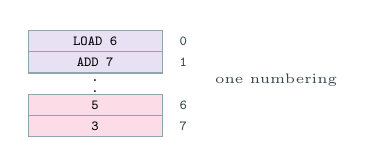
\begin{tikzpicture}
  \node[smallcell, fill=sViolet!18, minimum width=1.7cm] (o0) at (0,0.5) {LOAD 6};
  \node[smallcell, fill=sViolet!18, minimum width=1.7cm] at (0,0.23) {ADD 7};
  \node[smallcell, draw=none, minimum width=1.7cm] at (0,-0.04) {$\vdots$};
  \node[smallcell, fill=sPink!18, minimum width=1.7cm] at (0,-0.31) {5};
  \node[smallcell, fill=sPink!18, minimum width=1.7cm] at (0,-0.58) {3};
  \node[addr, font=\ttfamily\tiny, anchor=west] at (0.95,0.5) {0};
  \node[addr, font=\ttfamily\tiny, anchor=west] at (0.95,0.23) {1};
  \node[addr, font=\ttfamily\tiny, anchor=west] at (0.95,-0.31) {6};
  \node[addr, font=\ttfamily\tiny, anchor=west] at (0.95,-0.58) {7};
  \node[font=\tiny, text=nInk, anchor=west] at (1.4,0) {one numbering};
\end{tikzpicture}}

\newcommand{\diagDecimal}{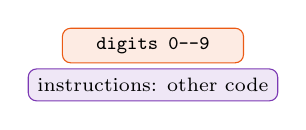
\begin{tikzpicture}
  \node[draw=AccentOrange, fill=AccentOrange!12, rounded corners=3pt, font=\ttfamily\scriptsize, minimum height=0.4cm,
    minimum width=2.3cm] at (0,0.28) {digits 0--9};
  \node[draw=ProgramPurple, fill=ProgramPurple!12, rounded corners=3pt, font=\scriptsize, minimum height=0.4cm,
    minimum width=2.3cm] at (0,-0.22) {instructions: other code};
\end{tikzpicture}}

\newcommand{\diagBinary}{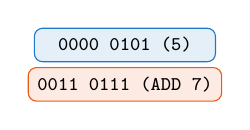
\begin{tikzpicture}
  \node[draw=StorageBlue, fill=StorageBlue!12, rounded corners=3pt, font=\ttfamily\scriptsize, minimum height=0.4cm,
    minimum width=2.3cm] at (0,0.28) {0000 0101 (5)};
  \node[draw=AccentOrange, fill=AccentOrange!12, rounded corners=3pt, font=\ttfamily\scriptsize, minimum height=0.4cm,
    minimum width=2.3cm] at (0,-0.22) {0011 0111 (ADD 7)};
\end{tikzpicture}}

\newcommand{\diagParallel}{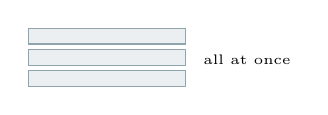
\begin{tikzpicture}
  \foreach \k in {0,1,2} {\draw[fill=nFill, draw=nLine] (0,{0.6-0.27*\k}) rectangle (2.0,{0.4-0.27*\k});}
  \node[font=\tiny, anchor=west] at (2.1,0.2) {all at once};
\end{tikzpicture}}

\newcommand{\diagDataflow}{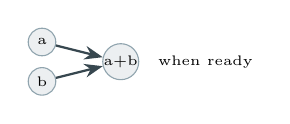
\begin{tikzpicture}[>=Stealth]
  \node[circle, draw=nLine, fill=nFill, minimum size=0.35cm, inner sep=0pt, font=\tiny] (a) at (0,0.3) {a};
  \node[circle, draw=nLine, fill=nFill, minimum size=0.35cm, inner sep=0pt, font=\tiny] (b) at (0,-0.2) {b};
  \node[circle, draw=nLine, fill=nFill, minimum size=0.4cm, inner sep=0pt, font=\tiny] (c) at (1.0,0.05) {a+b};
  \draw[->, thick, nInk] (a) -- (c); \draw[->, thick, nInk] (b) -- (c);
  \node[font=\tiny, anchor=west] at (1.35,0.05) {when ready};
\end{tikzpicture}}

\newcommand{\diagSequential}{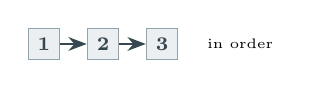
\begin{tikzpicture}[>=Stealth]
  \foreach \k in {1,2,3} {\node[draw=nLine, fill=nFill, text=nInk, minimum size=0.4cm, inner sep=0pt, font=\scriptsize\bfseries]
    (s\k) at ({0.75*\k-0.75},0.05) {\k};}
  \draw[->, thick, nInk] (s1) -- (s2); \draw[->, thick, nInk] (s2) -- (s3);
  \node[font=\tiny, anchor=west] at (1.95,0.05) {in order};
\end{tikzpicture}}

\newcommand{\diagMonolith}{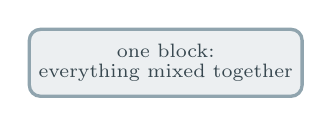
\begin{tikzpicture}
  \node[draw=nLine, very thick, rounded corners=4pt, fill=nFill, text=nInk, minimum width=2.6cm, minimum height=0.85cm,
    font=\scriptsize, align=center] {one block:\\[-1pt]everything mixed together};
\end{tikzpicture}}

\newcommand{\diagUnits}{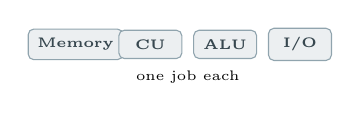
\begin{tikzpicture}
  \node[draw=nLine, fill=nFill, text=nInk, rounded corners=2pt, font=\tiny\bfseries, minimum width=0.8cm, minimum height=0.36cm] at (0,0.22) {Memory};
  \node[draw=nLine, fill=nFill, text=nInk, rounded corners=2pt, font=\tiny\bfseries, minimum width=0.8cm, minimum height=0.36cm] at (0.95,0.22) {CU};
  \node[draw=nLine, fill=nFill, text=nInk, rounded corners=2pt, font=\tiny\bfseries, minimum width=0.8cm, minimum height=0.36cm] at (1.9,0.22) {ALU};
  \node[draw=nLine, fill=nFill, text=nInk, rounded corners=2pt, font=\tiny\bfseries, minimum width=0.8cm, minimum height=0.36cm] at (2.85,0.22) {I/O};
  \node[font=\tiny] at (1.425,-0.2) {one job each};
\end{tikzpicture}}

% ---------- helpers for the CPU section ----------
\tikzset{
  reg/.style={draw=nLine, very thick, fill=white, text=nInk, rounded corners=2pt,
    minimum width=1.95cm, minimum height=0.55cm, inner sep=2pt, font=\ttfamily\scriptsize, align=center},
  cpuunit/.style={very thick, rounded corners=3pt, minimum width=1.2cm, minimum height=0.6cm,
    inner sep=2pt, font=\scriptsize\bfseries, align=center},
  hot/.style={aexec, label={[text=aExec, inner sep=1pt, font=\tiny]right:$\blacktriangleleft$}},
  hotdata/.style={aread},
  hotwrite/.style={awrite},
  hotalu/.style={aexec},
  fetcharrow/.style={-{Stealth}, very thick, DeepBlue, rounded corners=3pt},
  dataarrow/.style={-{Stealth}, very thick, DeepBlue, rounded corners=3pt},
  steplabel/.style={font=\tiny\bfseries, fill=white, inner sep=1pt},
}
% memory with the running example
% #1 highlighted instruction (0-3, -1 = none)  #2 text of cell 8  #3 highlighted data cell (6-8, 0 = none)
\newcommand{\mempanel}[3]{%
  \node[font=\scriptsize\bfseries, text=nInk] at (0,1.8) {Memory};
  \foreach \i/\t in {0/{0001 0110\ \ LOAD 6},1/{0011 0111\ \ ADD 7},2/{0010 1000\ \ STORE 8},3/{0111 0000\ \ HALT}} {
    \ifnum\i=#1
      \node[instrcell, minimum width=2.9cm, hot] (m\i) at (0,{1.35-0.45*\i}) {\t};
    \else
      \node[instrcell, minimum width=2.9cm] (m\i) at (0,{1.35-0.45*\i}) {\t};
    \fi
    \node[addr, anchor=east] at (-1.5,{1.35-0.45*\i}) {\i};
  }
  \node[memcell, draw=none, minimum width=2.9cm] at (0,-0.45) {$\vdots$};
  \foreach \i/\t/\y in {6/{0000 0101\ \ (5)}/-0.9,7/{0000 0011\ \ (3)}/-1.35,8/{#2}/-1.8} {
    \ifnum\i=#3
      \ifnum\i=8 \node[datacell, minimum width=2.9cm, hotwrite] (m\i) at (0,\y) {\t};\else \node[datacell, minimum width=2.9cm, hotdata] (m\i) at (0,\y) {\t};\fi
    \else
      \node[datacell, minimum width=2.9cm] (m\i) at (0,\y) {\t};
    \fi
    \node[addr, anchor=east] at (-1.5,\y) {\i};
  }
}
% the CPU, built up step by step
% #1 level: 0 empty, 1 +PC, 2 +IR, 3 +AC, 4 +ALU, 5 +CU   #2 PC   #3 IR   #4 AC   #5 extra ALU style
\newcommand{\cpupanel}[5]{%
  \node[draw=nLine, very thick, rounded corners=6pt, fill=nFill!50, minimum width=4.65cm,
    minimum height=3.85cm, anchor=west] (cpu) at (2.45,-0.2) {};
  \node[font=\scriptsize\bfseries, text=nInk, anchor=north west] at ([shift={(0.1,-0.06)}]cpu.north west) {CPU};
  \ifnum#1>0 \node[reg] (pc) at (3.65,0.95) {\textbf{PC}\ \ #2}; \fi
  \ifnum#1>1 \node[reg] (ir) at (3.65,0.0) {\textbf{IR}\\[-1pt]#3}; \fi
  \ifnum#1>2 \node[reg] (ac) at (3.65,-1.05) {\textbf{AC}\ \ #4}; \fi
  \ifnum#1>3 \node[cpuunit, draw=mygreen, fill=mygreen!18, #5] (alu) at (6.3,-1.05)
    {\textcolor{mygreen!60!black}{\faCalculator}\\[-1pt]ALU}; \fi
  \ifnum#1>4 \node[cpuunit, draw=AccentOrange, fill=AccentOrange!18] (cu) at (6.3,0.5)
    {\textcolor{AccentOrange}{\faCogs}\\[-1pt]CU}; \fi
}
% explanation slide: #1 title, #2 tikz body (memory + CPU), #3 right-hand column
\newcommand{\explainframe}[3]{%
\begin{frame}{#1}
  \begin{columns}[c,onlytextwidth]
    \column{0.58\textwidth}
      \centering
      \begin{tikzpicture}[>=Stealth, scale=0.92, every node/.append style={transform shape}]
        #2
      \end{tikzpicture}
    \column{0.4\textwidth}
      #3
  \end{columns}
\end{frame}}
% boxes for the right-hand column
\newcommand{\defbox}[1]{%
  \begin{beamercolorbox}[rounded=true,sep=0.1cm,wd=\linewidth]{block body example}
    \footnotesize #1
  \end{beamercolorbox}\vspace{0.06cm}}
\newcommand{\stepbox}[2]{%
  \begin{beamercolorbox}[rounded=true,sep=0.09cm,wd=\linewidth]{block body}
    \footnotesize\textbf{#1}\\ #2
  \end{beamercolorbox}\vspace{0.06cm}}
\newcommand{\phasename}[1]{%
  {\centering\footnotesize Name of this phase:\ \colorbox{DeepBlue}{\textcolor{white}{\textbf{#1}}}\par}}
% small tag above the CPU box: which instruction is being executed
\newcommand{\executing}[1]{%
  \node[font=\scriptsize\bfseries, text=AccentOrange, anchor=south east] at ([yshift=1pt]cpu.north east)
    {Executing: \texttt{#1}};}
\newcommand{\statebox}[1]{%
  {\centering\scriptsize\textcolor{DeepBlue}{\textbf{State:}}\ #1\par}}

\lstset{
  language=Python,
  basicstyle=\color{VSText}\ttfamily\footnotesize,
  keywordstyle=\color{VSPurple}\bfseries,
  stringstyle=\color{VSString},
  commentstyle=\color{VSComment}\itshape,
  numbers=left,
  numberstyle=\tiny\color{gray},
  stepnumber=1,
  breaklines=true,
  showstringspaces=false,
  xleftmargin=15pt,
  xrightmargin=5pt,
  frame=none
}

% MARIE assembly: line numbers start at 0, so a line number equals the memory address
\lstdefinelanguage{MARIE}{
  morekeywords={Load,Store,Add,Subt,Input,Output,Halt,Jump,Skipcond,DEC,HEX,ADR,LoadI,StoreI,AddI,JumpI,JnS,Clear,LoadImmi},
  sensitive=false,
  comment=[l]{/},
}
\lstdefinestyle{marie}{language=MARIE, firstnumber=0, basicstyle=\color{VSText}\ttfamily\scriptsize,
  keywordstyle=\color{VSBlue}\bfseries, commentstyle=\color{VSComment}\itshape,
  columns=fixed, basewidth=0.52em, keepspaces=true, breaklines=false, xleftmargin=12pt}

\BeforeBeginEnvironment{lstlisting}{%
  \begin{beamercolorbox}[rounded=true,sep=2mm,wd=\linewidth]{vscodelisting}%
  
\begin{tikzpicture}
    \fill[nLine] (0,0) circle (3pt);
    \fill[nLine] (0.35,0) circle (3pt);
    \fill[nLine] (0.70,0) circle (3pt);
  \end{tikzpicture}%
  \vspace{-0.2cm}%
}
\AfterEndEnvironment{lstlisting}{\end{beamercolorbox}}

% =====================================================================
%  Day 2 helpers
% =====================================================================

% ---------- MARIE datapath, drawn like the Data Path view of MARIE.js ----------
% \busdiagram[values]{source}{destination}{extra TikZ}
%   source (Read, blue) and destination (Write, red): ir, out, in, ac, mbr, pc, mar, mem, none
%   values: ir=, out=, in=, ac=, mbr=, pc=, mar=, mem= (contents of M[MAR]), step= (0-7, -1 = none)
\definecolor{ReadBlue}{HTML}{1E88E5}
\definecolor{WriteRed}{HTML}{E53935}
\definecolor{BusGreen}{HTML}{B0BEC5}% the bus: neutral
\tikzset{
  dpreg/.style={draw=nLine, thick, fill=white, text=nInk, minimum width=1.1cm, minimum height=0.46cm,
    inner sep=1pt, font=\ttfamily\scriptsize},
  dpname/.style={font=\tiny, text=nInk, above=0pt, inner sep=1pt},
  dpwire/.style={thin, nLight},
  dpmem/.style={draw=nLine, very thick, fill=nFill, rounded corners=3pt,
    minimum width=1.3cm, minimum height=0.95cm, font=\scriptsize\bfseries, align=center},
  srcreg/.style={aread},
  dstreg/.style={awrite},
}
\pgfkeys{/dp/.is family, /dp,
  ir/.initial={0000}, out/.initial={0000}, in/.initial={0000}, ac/.initial={0000},
  mbr/.initial={0000}, pc/.initial={000}, mar/.initial={000}, mem/.initial={0000},
  step/.initial={-1}}
\newcommand{\dpv}[1]{\pgfkeysvalueof{/dp/#1}}
\newcommand{\busdiagram}[4][]{%
  \begingroup
  \pgfkeys{/dp, ir=0000, out=0000, in=0000, ac=0000, mbr=0000, pc=000, mar=000, mem=0000, step=-1, #1}%
  \begin{tikzpicture}[>=Stealth]
    \tikzset{bd-mem/.style={}, bd-mar/.style={}, bd-pc/.style={}, bd-mbr/.style={},
      bd-ac/.style={}, bd-ir/.style={}, bd-in/.style={}, bd-out/.style={}, bd-none/.style={}}
    \tikzset{bd-#2/.style={srcreg}}
    \tikzset{bd-#3/.style={dstreg}}
    % ----- control unit -----
    \node[draw=DeepBlue!80, thick, fill=white, minimum width=1.3cm, minimum height=2.95cm,
      anchor=north west] (cu) at (-2.4,2.0) {};
    \node[font=\tiny, text=DeepBlue, anchor=north west, below=1pt] at (cu.south west) {Control unit};
    \node[font=\tiny, text=DeepBlue!80, anchor=east] at (-1.15,1.75) {Read};
    \node[font=\tiny, text=DeepBlue!80, anchor=east] at (-1.15,-0.6) {Write};
    \node[font=\tiny, text=DeepBlue!80, anchor=east] at (-1.15,0.05) {AC<0};
    \node[font=\tiny, text=DeepBlue!80, anchor=east] at (-1.15,-0.15) {AC=0};
    \node[font=\tiny, text=DeepBlue!80] at (-2.0,1.3) {Step};
    \foreach \k in {0,...,7} {
      \pgfmathtruncatemacro{\cur}{\dpv{step}}
      \ifnum\k=\cur
        \fill[AccentOrange] (-2.0,{1.1-0.15*\k}) circle (0.065);
      \else
        \fill[DeepBlue!30] (-2.0,{1.1-0.15*\k}) circle (0.035);
      \fi
    }
    % ----- memory -----
    \node[draw=DeepBlue!80, thick, fill=white, minimum width=1.5cm, minimum height=2.95cm,
      anchor=north west, bd-mem] (mem) at (10.4,2.0) {};
    \node[font=\tiny, text=DeepBlue, anchor=north west, below=1pt] at (mem.south west) {Main memory};
    \node[font=\ttfamily\tiny, text=DeepBlue!80] at (11.15,0.75) {M[MAR]};
    \node[font=\ttfamily\scriptsize] at (11.15,0.5) {\dpv{mem}};
    % ----- faint control wires (one Read and one Write wire per device) -----
    \draw[dpwire] (-1.1,1.75) -- (10.4,1.75);
    \draw[dpwire] (-1.1,-0.6) -- (10.4,-0.6);
    \foreach \x in {0.6,2.0,3.4,4.8,6.2,7.6,9.0} {
      \draw[dpwire] (\x-0.25,1.75) -- (\x-0.25,1.18);
      \draw[dpwire] (\x+0.3,-0.6) -- (\x+0.3,0.72);
    }
    % ----- bus (drawn first, registers on top) -----
    \foreach \x in {0.6,2.0,3.4,4.8,6.2,7.6,9.0}
      \draw[line width=2.6pt, BusGreen] (\x,0.72) -- (\x,-0.35);
    \draw[line width=2.6pt, BusGreen] (0.6-0.045,-0.35) -- (10.4,-0.35);
    % ----- ALU between AC and MBR, with its links and the flag wires to the CU -----
    \draw[thin, DeepBlue!40] (4.45,0.05) -- (-1.1,0.05);
    \draw[thin, DeepBlue!40] (4.45,-0.15) -- (-1.1,-0.15);
    \draw[thick, DeepBlue!70, fill=white] (5.0,0.47) -- (5.42,0.47) -- (5.5,0.37) -- (5.58,0.47) -- (6.0,0.47)
      -- (5.72,0.05) -- (5.28,0.05) -- cycle;
    \node[font=\tiny, text=DeepBlue!80] at (5.5,0.22) {ALU};
    \draw[thick, DeepBlue!60] (5.2,0.72) -- (5.2,0.47);
    \draw[thick, DeepBlue!60] (5.8,0.72) -- (5.8,0.47);
    \draw[thick, DeepBlue!60] (5.5,0.05) -- (5.5,-0.1) -- (4.45,-0.1) |- (4.45,0.72);
    % ----- registers -----
    \foreach \n/\x/\lab in {ir/0.6/IR, out/2.0/OUT, in/3.4/IN, ac/4.8/AC, mbr/6.2/MBR, pc/7.6/PC, mar/9.0/MAR} {
      \node[dpreg, bd-\n] (\n) at (\x,0.95) {\dpv{\n}};
      \node[dpname] at (\n.north) {\lab};
      \coordinate (\n-port) at (\n.south);
      \coordinate (\n-bus) at (\x,-0.35);
    }
    \coordinate (mem-port) at (10.4,-0.35);
    \coordinate (mem-bus) at (10.4,-0.35);
    % IR is decoded by the CU; MAR selects the memory cell
    \draw[thick, BusGreen, -{Stealth}] (ir.west) -- (-1.1,0.95);
    \draw[thick, BusGreen, -{Stealth}] (mar.east) -- (10.4,0.95);
    % ----- active Read and Write signals -----
    \ifstrequal{#2}{none}{}{%
      \ifstrequal{#2}{mem}
        {\draw[line width=1.3pt, ReadBlue, -{Stealth}] (-1.1,1.75) -- (10.4,1.75);}
        {\draw[line width=1.3pt, ReadBlue, -{Stealth}] (-1.1,1.75) -| ($(#2.north)+(-0.25,0)$);}}
    \ifstrequal{#3}{none}{}{%
      \ifstrequal{#3}{mem}
        {\draw[line width=1.3pt, WriteRed, -{Stealth}] (-1.1,-0.6) -- (10.4,-0.6);}
        {\draw[line width=1.3pt, WriteRed, -{Stealth}] (-1.1,-0.6) -| ($(#3.south)+(0.3,0)$);}}
    % ----- the value travelling along the bus -----
    \ifstrequal{#2}{none}{}{\ifstrequal{#3}{none}{}{%
      \draw[line width=3pt, nInk] (#2-port) -- (#2-bus) -- (#3-bus) -- (#3-port);
      \draw[line width=1.5pt, white, dash pattern=on 1.5pt off 1.5pt] (#2-port) -- (#2-bus) -- (#3-bus) -- (#3-port);}}
    #4
  \end{tikzpicture}%
  \endgroup}

% legend for the colours of the data path
\newcommand{\dplegend}{%
  {\tiny\tikz[baseline=-0.6ex]\draw[aread] (0,-0.08) rectangle (0.4,0.12);\ \textbf{Read}: puts its value on the bus
  \qquad\tikz[baseline=-0.6ex]\draw[awrite] (0,-0.08) rectangle (0.4,0.12);\ \textbf{Write}: stores the value from the bus
  \qquad\tikz[baseline=-0.6ex]{\draw[line width=3pt, nInk] (0,0) -- (0.5,0);\draw[line width=1.5pt, white, dash pattern=on 1.5pt off 1.5pt] (0,0) -- (0.5,0);}\ the value travelling on the bus}}

% one step of an instruction: data path on top, explanation below
% #1 title, #2 source, #3 destination, #4 values (keys), #5 explanation
\newcommand{\stepframe}[5]{%
\begin{frame}{#1}
  \begin{center}
    \resizebox{0.8\textwidth}{!}{\busdiagram[#4]{#2}{#3}{}}\\[0.02cm]
    \dplegend
  \end{center}
  \vspace{-0.1cm}
  \begin{center}
    \begin{minipage}{0.8\textwidth}
      #5
    \end{minipage}
  \end{center}
\end{frame}}

% ---------- timeline of clock steps ----------
% #1 fetch steps, #2 execute steps, #3 label on the right
\newcommand{\steptimeline}[3]{%
  \begin{tikzpicture}
    \foreach \i in {1,...,#1}
      \node[draw=white, fill=sAmber, text=black, font=\tiny\bfseries, minimum width=0.62cm,
        minimum height=0.45cm, inner sep=0pt] at ({0.62*(\i-1)},0) {T\the\numexpr\i-1\relax};
    \foreach \i in {1,...,#2}
      \node[draw=white, fill=sTeal, text=white, font=\tiny\bfseries, minimum width=0.62cm,
        minimum height=0.45cm, inner sep=0pt] at ({0.62*(#1+\i-1)},0) {T\the\numexpr#1+\i-1\relax};
    \node[anchor=west, font=\scriptsize] at ({0.62*(#1+#2)-0.25},0) {#3};
  \end{tikzpicture}}

% legend for the timeline colours
\newcommand{\timelinelegend}{%
  {\tiny\textcolor{sAmber}{\rule{0.25cm}{0.2cm}}\ fetch
  \qquad\textcolor{sTeal}{\rule{0.25cm}{0.2cm}}\ execute}}

% ---------- small pieces for the addressing-mode slides ----------
\tikzset{
  mcell/.style={draw=nLine, minimum width=1.5cm, minimum height=0.42cm, inner sep=1pt,
    font=\ttfamily\scriptsize, align=center, fill=white, text=nInk},
  mcellhot/.style={mcell, fill=sPink!25, draw=sPink, very thick},
  mcellptr/.style={mcell, fill=sIndigo!20, draw=sIndigo, very thick},
  instrbox/.style={draw=sViolet, very thick, fill=sViolet!15, rounded corners=2pt,
    minimum height=0.5cm, inner sep=3pt, font=\ttfamily\scriptsize},
  ptrarrow/.style={-{Stealth}, very thick, nInk},
  valarrow/.style={-{Stealth}, very thick, nInk},
}

% task header box (same look as on Day 1)
% #1 form and time, #2 short instruction
\newcommand{\taskhead}[2]{%
  \begin{beamercolorbox}[rounded=true,sep=0.12cm,wd=\linewidth]{block body example}
    \small\textbf{#1}\\[0.04cm]
    \footnotesize #2
  \end{beamercolorbox}\vspace{0.1cm}}

% highlighted key message at the bottom of a slide
\newcommand{\keymsg}[1]{%
  \begin{beamercolorbox}[rounded=true,sep=0.1cm,wd=\textwidth]{block body example}
    \centering\footnotesize #1
  \end{beamercolorbox}}

% register transfer written in text: \mo{MAR}{PC} gives MAR <- PC
\newcommand{\mo}[2]{\texttt{#1\,$\leftarrow$\,#2}}

% plain listings (x86, RISC-V) without Python highlighting
\lstdefinelanguage{plain}{}
\lstdefinestyle{asm}{language=plain, basicstyle=\color{VSText}\ttfamily\scriptsize, numbers=none,
  columns=fixed, basewidth=0.52em, keepspaces=true, xleftmargin=6pt}

\title{Computer Hardware}
\subtitle{Inside the Processor}
\author{Ksawery Możdżyński}
\date{}

\begin{document}

\begin{frame}
  \titlepage
\end{frame}

\begin{frame}{Agenda For Today}
  \Large
  \begin{itemize}
    \item[\textcolor{DeepBlue}{\faMapMarker}] \textbf{1. Addressing Modes} \\
    \textcolor{gray}{\small Direct and indirect addressing, arrays, and immediate values}
    \vspace{0.25cm}

    \item[\textcolor{DeepBlue}{\faArrowRight}] \textbf{2. How the CPU Talks to Memory} \\
    \textcolor{gray}{\small MAR, MBR, the bus, micro-operations, instruction steps, and the von Neumann bottleneck}
    \vspace{0.25cm}

    \item[\textcolor{DeepBlue}{\faSitemap}] \textbf{3. The Control Unit} \\
    \textcolor{gray}{\small How control signals are generated: hardwired and microprogrammed control}
    \vspace{0.25cm}

    \item[\textcolor{DeepBlue}{\faBalanceScale}] \textbf{4. RISC and CISC} \\
    \textcolor{gray}{\small Operand sources, instruction length, a comparison exercise, and RISC/CISC today}
  \end{itemize}
\end{frame}

% ---------- Recap of Day 1 ----------
\begin{frame}{Where we stopped on Day 1}
  \begin{columns}[c,onlytextwidth]
    \column{0.45\textwidth}
      \centering
      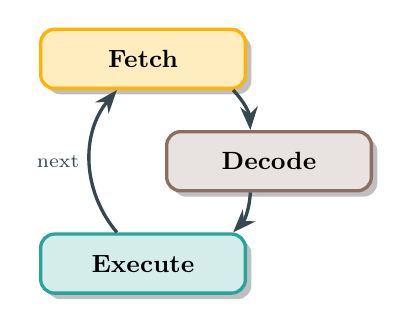
\begin{tikzpicture}[>=Stealth,
          phase/.style={very thick, rounded corners=5pt, minimum width=2.6cm, minimum height=0.75cm,
            align=center, font=\small\bfseries, drop shadow}]
        \node[phase, draw=sAmber, fill=sAmber!25] (f) at (0,1.3) {Fetch};
        \node[phase, draw=sBrown, fill=sBrown!20] (d) at (1.6,0) {Decode};
        \node[phase, draw=sTeal, fill=sTeal!20] (e) at (0,-1.3) {Execute};
        \draw[->, very thick, nInk] (f) to[bend left=20] (d);
        \draw[->, very thick, nInk] (d) to[bend left=20] (e);
        \draw[->, very thick, nInk] (e) to[bend left=40] node[left, font=\scriptsize] {next} (f);
      \end{tikzpicture}
    \column{0.52\textwidth}
      \begin{beamercolorbox}[rounded=true,sep=0.1cm,wd=\linewidth]{block body}
        \footnotesize
        \textbf{PC} -- points to the next instruction\\[2pt]
        \textbf{IR} -- holds the instruction being executed\\[2pt]
        \textbf{AC} -- holds the working value\\[2pt]
        \textbf{ALU} calculates, \textbf{CU} directs
      \end{beamercolorbox}
      \vspace{0.15cm}
      \footnotesize\textbf{MARIE instructions you know}\\[0.05cm]
      \texttt{Load}, \texttt{Store}, \texttt{Add}, \texttt{Subt}, \texttt{Input}, \texttt{Output},
      \texttt{Jump}, \texttt{Skipcond}, \texttt{Halt}
  \end{columns}
  \vfill
  \keymsg{Day 1: \textbf{what} the processor does. \ Today: \textbf{how} it does it inside.}
\end{frame}

% =====================================================================
\section{Addressing modes}
% =====================================================================

\begin{frame}{How does an instruction point to its data?}
  \begin{beamercolorbox}[rounded=true,sep=0.12cm,wd=\textwidth]{block body}
    \centering\small
    In memory, \texttt{Load X} (with \texttt{X} at address 4) is stored as \texttt{1004}: opcode \texttt{1} and address \texttt{004}.
    The address is \textbf{part of the instruction}.
  \end{beamercolorbox}
  \vspace{0.3cm}
  \begin{center}
    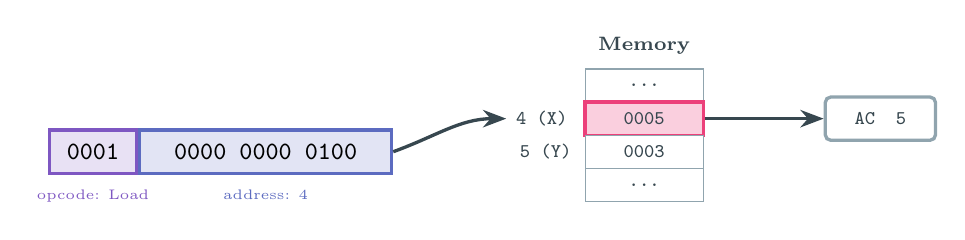
\begin{tikzpicture}[>=Stealth]
      \node[draw=sViolet, fill=sViolet!18, very thick, minimum width=1.1cm, minimum height=0.55cm,
        font=\ttfamily\small] (op) at (0,0) {0001};
      \node[draw=sIndigo, fill=sIndigo!18, very thick, minimum width=3.2cm, minimum height=0.55cm,
        font=\ttfamily\small, right=0pt of op] (ad) {0000 0000 0100};
      \node[font=\tiny, text=sViolet, below=2pt of op] {opcode: Load};
      \node[font=\tiny, text=sIndigo, below=2pt of ad] {address: 4};
      \node[mcell] (c5) at (7,0.84) {\dots};
      \node[mcellhot] (c6) at (7,0.42) {0005};
      \node[mcell] (c7) at (7,0) {0003};
      \node[mcell] (c8) at (7,-0.42) {\dots};
      \node[addr, anchor=east] (l6) at (6.15,0.42) {4 (\texttt{X})};
      \node[addr, anchor=east] at (6.2,0) {5 (\texttt{Y})};
      \node[font=\scriptsize\bfseries, text=nInk] at (7,1.35) {Memory};
      \node[reg, minimum width=1.4cm] (ac) at (10,0.42) {\textbf{AC}\ \ 5};
      \draw[ptrarrow] (ad.east) to[out=20, in=180] (l6.west);
      \draw[valarrow] (c6.east) -- (ac.west);
    \end{tikzpicture}
  \end{center}
  \vspace{0.2cm}
  \begin{columns}[T,onlytextwidth]
    \column{0.48\textwidth}
      \defbox{The assembler writes the address into the instruction when it translates the program.
        After that, the address \textbf{never changes}.}
    \column{0.48\textwidth}
      \defbox{This way of pointing to the data is called \textbf{direct addressing}.}
  \end{columns}
\end{frame}

\begin{frame}[fragile]{A problem: adding up an array}
  \begin{beamercolorbox}[rounded=true,sep=0.1cm,wd=\textwidth]{block body}
    \centering\small
    Five numbers are stored in neighbouring cells \texttt{A1}\dots\texttt{A5}. We can add them one by one.
  \end{beamercolorbox}
  \vspace{0.18cm}
  \begin{columns}[T,onlytextwidth]
    \column{0.43\textwidth}
      \footnotesize\textbf{A direct solution:}
\begin{lstlisting}[style=marie]
Load A1
Add  A2
Add  A3
Add  A4
Add  A5
Store Sum
\end{lstlisting}
      \scriptsize The program works, but it contains one instruction for every array element.
    \column{0.47\textwidth}
      \centering
      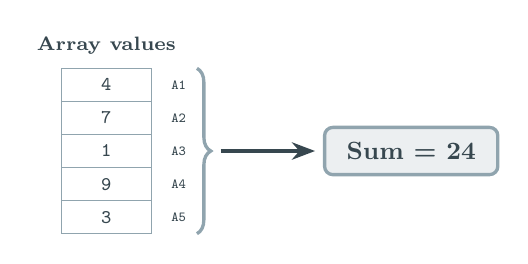
\begin{tikzpicture}[>=Stealth]
        \node[font=\scriptsize\bfseries, text=nInk] at (0,0.5) {Array values};
        \foreach \i/\v in {0/4,1/7,2/1,3/9,4/3} {
          \node[mcell, minimum width=1.15cm] at (0,{-0.42*\i}) {\v};
          \node[addr, anchor=west, font=\ttfamily\tiny] at (0.7,{-0.42*\i}) {A\the\numexpr\i+1\relax};
        }
        \draw[decorate, decoration={brace, amplitude=5pt}, very thick, nLine]
          (1.15,0.21) -- (1.15,-1.89);
        \draw[valarrow] (1.45,-0.84) -- (2.65,-0.84);
        \node[draw=nLine, fill=nFill, text=nInk, very thick, rounded corners=3pt,
          minimum width=2.2cm, minimum height=0.6cm, font=\small\bfseries, anchor=west] at (2.75,-0.84) {Sum = 24};
      \end{tikzpicture}
  \end{columns}
  \vfill
  \begin{beamercolorbox}[rounded=true,sep=0.11cm,wd=\textwidth]{block body example}
    \centering\small
    The result is $4+7+1+9+3=24$.
  \end{beamercolorbox}
\end{frame}

\begin{frame}[fragile]{The problem with repeating instructions}
  \begin{beamercolorbox}[rounded=true,sep=0.1cm,wd=\textwidth]{block body}
    \centering\small
    The direct solution works, but it does not scale. What if the array has 100 or 1000 elements?
  \end{beamercolorbox}
  \vspace{0.18cm}
  \begin{columns}[T,onlytextwidth]
    \column{0.42\textwidth}
      \footnotesize\textbf{A first attempt at a loop:}
\begin{lstlisting}[style=marie]
Loop, Load Sum
      Add A1   / always A1!
      Store Sum
      Jump Loop
\end{lstlisting}
    \column{0.5\textwidth}
      \begin{beamercolorbox}[rounded=true,sep=0.12cm,wd=\linewidth]{block body example}
        \footnotesize
        The loop repeats, but it keeps adding the value from \textbf{A1}. The address in \texttt{Add A1}
        is fixed inside the instruction.
      \end{beamercolorbox}
      \vspace{0.1cm}
      \begin{beamercolorbox}[rounded=true,sep=0.12cm,wd=\linewidth]{block body}
        \footnotesize
        To walk through an array, we need an address that can \textbf{change while the program runs}.
      \end{beamercolorbox}
  \end{columns}
  \vfill
  \begin{alertblock}{The next idea}
    \centering\small Keep the address in a memory cell, where the program can change it.
  \end{alertblock}
\end{frame}

\begin{frame}{The instruction decides what a value means}
  \begin{columns}[c,onlytextwidth]
    \column{0.45\textwidth}
      \centering
      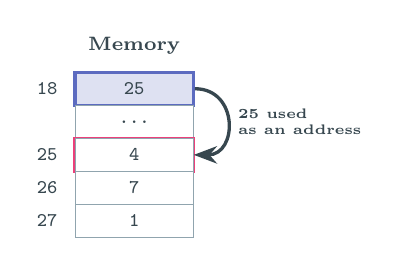
\begin{tikzpicture}[>=Stealth]
        \node[font=\scriptsize\bfseries, text=nInk] at (0,0.55) {Memory};
        \node[mcellptr] (p) at (0,0) {25};
        \node[mcell] at (0,-0.42) {\dots};
        \alt<2>{\node[mcellhot] (a) at (0,-0.84) {4};}{\node[mcell] (a) at (0,-0.84) {4};}
        \node[mcell] at (0,-1.26) {7};
        \node[mcell] at (0,-1.68) {1};
        \node[addr, anchor=east] at (-0.85,0) {18};
        \node[addr, anchor=east] at (-0.85,-0.84) {25};
        \node[addr, anchor=east] at (-0.85,-1.26) {26};
        \node[addr, anchor=east] at (-0.85,-1.68) {27};
        \draw<2>[ptrarrow] (p.east) to[out=0, in=0, looseness=1.7]
          node[right, font=\tiny\bfseries, align=left] {25 used\\as an address} (a.east);
      \end{tikzpicture}
    \column{0.52\textwidth}
      \begin{beamercolorbox}[rounded=true,sep=0.1cm,wd=\linewidth]{block body}
        \footnotesize\textbf{\texttt{Load 18}} \ (direct)\\[0.03cm]
        Takes the value from cell 18 and treats it as \textbf{data}.\\[0.03cm]
        \textcolor{DeepBlue}{\textbf{Result:}} \texttt{AC = 25}
      \end{beamercolorbox}
      \vspace{0.1cm}
      \uncover<2>{%
      \begin{beamercolorbox}[rounded=true,sep=0.1cm,wd=\linewidth]{block body example}
        \footnotesize\textbf{\texttt{LoadI 18}} \ (indirect)\\[0.03cm]
        Takes the value from cell 18 and treats it as an \textbf{address}:
        goes to cell 25 and takes the value from there.\\[0.03cm]
        \textcolor{DeepBlue}{\textbf{Result:}} \texttt{AC = 4}
      \end{beamercolorbox}}
  \end{columns}
  \vfill
  \keymsg{The memory does not know what 25 means. \textbf{The instruction decides}: data or address.}
\end{frame}

\begin{frame}{\texttt{LoadI 18} step by step: two memory reads}
  \begin{columns}[c,onlytextwidth]
    \column{0.55\textwidth}
      \centering
      \begin{tikzpicture}[>=Stealth]
        \node[font=\scriptsize\bfseries, text=nInk] at (0,0.55) {Memory};
        \node[mcellptr] (p) at (0,0) {25};
        \node[mcell] at (0,-0.42) {\dots};
        \alt<2>{\node[mcellhot] (a) at (0,-0.84) {4};}{\node[mcell] (a) at (0,-0.84) {4};}
        \node[mcell] at (0,-1.26) {7};
        \node[addr, anchor=east] at (-0.85,0) {18};
        \node[addr, anchor=east] at (-0.85,-0.84) {25};
        \node[addr, anchor=east] at (-0.85,-1.26) {26};
        \node[draw=nInk, very thick, rounded corners=6pt, fill=nFill, minimum width=2.4cm,
          minimum height=1.6cm] (cpu) at (4,-0.4) {};
        \node[font=\scriptsize\bfseries, text=nInk, anchor=north west] at (cpu.north west) {CPU};
        \node[reg, minimum width=1.6cm] (ac) at (4,-0.6) {\textbf{AC}\ \ \only<1>{?}\only<2>{4}};
        \draw<1>[ptrarrow] (p.east) -- node[midway, above=1pt, font=\bfseries\small, text=nInk] {1} (cpu.west |- p.east);
        \draw<2>[ptrarrow, opacity=0.3] (p.east) -- (cpu.west |- p.east);
        \draw<2>[valarrow] (a.east) -- node[midway, below=1pt, font=\bfseries\small, text=nInk] {2} (cpu.west |- a.east);
      \end{tikzpicture}
    \column{0.42\textwidth}
      \begin{beamercolorbox}[rounded=true,sep=0.1cm,wd=\linewidth]{block body example}
        \centering\small\textbf{Instruction being executed}\\[0.05cm]
        \texttt{LoadI 18}
      \end{beamercolorbox}
      \vspace{0.08cm}
      \stepbox{Step 1}{The CPU reads cell 18 and gets \textbf{25}. \texttt{LoadI} treats it as an \textbf{address}.}
      \uncover<2>{\stepbox{Step 2}{The CPU reads cell \textbf{25} and gets \textbf{4}. The value goes into the AC.}
      \statebox{\texttt{AC = 4}}}
  \end{columns}
  \vfill
  \keymsg{More memory reads mean more work for the processor. We will measure this later today.}
\end{frame}

\begin{frame}{Indirect instructions in MARIE}
  \begin{center}
    \scriptsize
    \renewcommand{\arraystretch}{1.25}
    \begin{tabular}{llcl}
      \toprule
      \textbf{Instruction} & \textbf{Effect} & \textbf{Opcode} & \textbf{In words} \\
      \midrule
      \texttt{LoadI X}  & $\mathsf{AC}\leftarrow\mathsf{M}[\mathsf{M}[X]]$ & D & bring the value from the address stored in \texttt{X} \\
      \texttt{StoreI X} & $\mathsf{M}[\mathsf{M}[X]]\leftarrow\mathsf{AC}$ & E & write the AC to the address stored in \texttt{X} \\
      \texttt{AddI X}   & $\mathsf{AC}\leftarrow\mathsf{AC}+\mathsf{M}[\mathsf{M}[X]]$ & B & add the value from the address stored in \texttt{X} \\
      \texttt{JumpI X}  & $\mathsf{PC}\leftarrow\mathsf{M}[X]$ & C & jump to the address stored in \texttt{X} \\
      \bottomrule
    \end{tabular}
  \end{center}
  \vspace{0.3cm}
  \begin{columns}[T,onlytextwidth]
    \column{0.48\textwidth}
      \defbox{The letter \textbf{I} stands for \textbf{indirect}.}
    \column{0.48\textwidth}
      \defbox{$\mathsf{M}[\mathsf{M}[X]]$: first read cell $X$, then use what you found as an address.}
  \end{columns}
\end{frame}

\begin{frame}[fragile]{A program that walks through an array}
  \begin{columns}[T,onlytextwidth]
    \column{0.44\textwidth}
\begin{lstlisting}[style=marie]
Loop,  LoadI Addr    / read element
       Skipcond 800  / > 0? skip Halt
       Halt
       Output
       Load Addr
       Add One
       Store Addr    / Addr + 1
       Jump Loop
One,   DEC 1
Addr,  ADR Arr       / address of Arr
Arr,   DEC 4
       DEC 7
       DEC 1
       DEC 0         / end of array
\end{lstlisting}
    \column{0.53\textwidth}
      \stepbox{\texttt{ADR Arr}}{The assembler puts the \textbf{address} of \texttt{Arr} into \texttt{Addr}.}
      \stepbox{\texttt{LoadI Addr}}{reads the value from the address stored in \texttt{Addr}.}
      \stepbox{\texttt{Load}, \texttt{Add}, \texttt{Store}}{increase the address in \texttt{Addr} by 1,
        so the next pass reads the next cell.}
      \stepbox{\texttt{Skipcond 800}}{The array ends with \textbf{0}: then \texttt{Halt} is not skipped
        and the program stops. (Elements must be greater than 0.)}
  \end{columns}
  \vfill
  \keymsg{The program prints \textbf{4, 7, 1}: every element of the array, with one \texttt{LoadI} instruction.}
\end{frame}

\begin{frame}{Walking through the array, pass by pass}
  \begin{columns}[c,onlytextwidth]
    \column{0.4\textwidth}
      \centering
      \begin{tikzpicture}[>=Stealth]
        \node[font=\scriptsize\bfseries, text=nInk] at (0,0.55) {Memory};
        \only<1>{\node[mcellptr] (ad) at (0,0) {10};}
        \only<2>{\node[mcellptr] (ad) at (0,0) {11};}
        \only<3>{\node[mcellptr] (ad) at (0,0) {12};}
        \only<4>{\node[mcellptr] (ad) at (0,0) {13};}
        \node[addr, anchor=east] at (-0.85,0) {9 (\textbf{Addr})};
        \alt<1>{\node[mcellhot] (e0) at (0,-0.60) {4};}{\node[mcell] (e0) at (0,-0.60) {4};}
        \node[addr, anchor=east] at (-0.85,-0.60) {10 (\textbf{Arr})};
        \alt<2>{\node[mcellhot] (e1) at (0,-1.02) {7};}{\node[mcell] (e1) at (0,-1.02) {7};}
        \node[addr, anchor=east] at (-0.85,-1.02) {11};
        \alt<3>{\node[mcellhot] (e2) at (0,-1.44) {1};}{\node[mcell] (e2) at (0,-1.44) {1};}
        \node[addr, anchor=east] at (-0.85,-1.44) {12};
        \alt<4>{\node[mcellhot] (e3) at (0,-1.86) {0};}{\node[mcell] (e3) at (0,-1.86) {0};}
        \node[addr, anchor=east] at (-0.85,-1.86) {13};
        \node[font=\tiny, anchor=west, text=gray] at (0.85,-1.86) {end of array};
        \draw<1>[ptrarrow] (ad.east) to[out=0, in=0, looseness=1.4] (e0.east);
        \draw<2>[ptrarrow] (ad.east) to[out=0, in=0, looseness=1.4] (e1.east);
        \draw<3>[ptrarrow] (ad.east) to[out=0, in=0, looseness=1.4] (e2.east);
        \draw<4>[ptrarrow] (ad.east) to[out=0, in=0, looseness=1.4] (e3.east);
      \end{tikzpicture}
    \column{0.57\textwidth}
      \centering
      \scriptsize
      \renewcommand{\arraystretch}{1.25}
      \begin{tabular}{cccc}
        \toprule
        \textbf{Pass} & \textbf{Value in \texttt{Addr}} & \textbf{\texttt{LoadI Addr} reads} & \textbf{Printed} \\
        \midrule
        \uncover<1->{1} & \uncover<1->{\texttt{10}} & \uncover<1->{\texttt{4}} & \uncover<1->{4} \\
        \uncover<2->{2} & \uncover<2->{\texttt{11}} & \uncover<2->{\texttt{7}} & \uncover<2->{7} \\
        \uncover<3->{3} & \uncover<3->{\texttt{12}} & \uncover<3->{\texttt{1}} & \uncover<3->{1} \\
        \uncover<4->{4} & \uncover<4->{\texttt{13}} & \uncover<4->{\texttt{0}} & \uncover<4->{-- (stop)} \\
        \bottomrule
      \end{tabular}\\[0.15cm]
      \uncover<4->{\raggedright\scriptsize Pass 4 reads \textbf{0}: \texttt{Skipcond} does not skip, so \texttt{Halt} runs.}
  \end{columns}
  \vfill
  \scriptsize\centering The assembler placed \texttt{Arr} at address 10, so \texttt{ADR Arr} put 10 into \texttt{Addr}.\par\vspace{0.05cm}
  \keymsg{The instruction \texttt{LoadI Addr} never changes. Only the \textbf{number stored in \texttt{Addr}} changes.}
\end{frame}

\begin{frame}[fragile]{Exercise 1: sum of an array}
  \begin{columns}[T,onlytextwidth]
    \column{0.36\textwidth}
\begin{lstlisting}[style=marie, numbers=none]
Sum,   DEC 0
One,   DEC 1
Addr,  ADR Arr / address of Arr
Arr,   DEC 4
       DEC 7
       DEC 1
       DEC 9
       DEC 3
       DEC 0   / end of array
\end{lstlisting}
      \scriptsize The data part of the program. Write the code above it.
    \column{0.61\textwidth}
      \taskhead{Task}{Write the program in MARIE.js.}
      \footnotesize
      \begin{enumerate}\setlength{\itemsep}{3pt}
        \item Change the program from the previous slides: instead of printing every element,
          \textbf{add them up} and print only the sum.
        \item Read the elements with \texttt{LoadI Addr}.
        \item Test: the program should print \textbf{24}.
      \end{enumerate}
      \vspace{0.05cm}
      \begin{beamercolorbox}[rounded=true,sep=0.1cm,wd=\linewidth]{block body}
        \scriptsize
        \textbf{Hint:} the loop ends the same way as in the printing program: on the value 0.
      \end{beamercolorbox}
  \end{columns}
\end{frame}

\begin{frame}[fragile]{Solution: sum of an array}
  \begin{columns}[T,onlytextwidth]
    \column{0.5\textwidth}
\begin{lstlisting}[style=marie]
Loop,  LoadI Addr    / read element
       Skipcond 800  / > 0? skip Jump
       Jump Done
       Add Sum       / element + Sum
       Store Sum
       Load Addr
       Add One
       Store Addr    / Addr + 1
       Jump Loop
\end{lstlisting}
    \column{0.47\textwidth}
\begin{lstlisting}[style=marie, firstnumber=9]
Done,  Load Sum
       Output
       Halt
Sum,   DEC 0
One,   DEC 1
Addr,  ADR Arr       / address of Arr
Arr,   DEC 4
       DEC 7
       DEC 1
       DEC 9
       DEC 3
       DEC 0         / end of array
\end{lstlisting}
  \end{columns}
  \vfill
  \keymsg{\textbf{Idea:} each pass reads the element at the address stored in \texttt{Addr}, adds it to \texttt{Sum}
    and increases \texttt{Addr} by 1, until it reads 0.}
\end{frame}

\begin{frame}[fragile]{Exercise 2: the largest element}
  \begin{columns}[T,onlytextwidth]
    \column{0.36\textwidth}
\begin{lstlisting}[style=marie, numbers=none]
Max,   DEC 0
One,   DEC 1
Addr,  ADR Arr / address of Arr
Arr,   DEC 4
       DEC 7
       DEC 1
       DEC 9
       DEC 3
       DEC 0   / end of array
\end{lstlisting}
      \scriptsize The data part of the program. Write the code above it.
    \column{0.61\textwidth}
      \taskhead{Task}{Write the program in MARIE.js.}
      \footnotesize
      \begin{enumerate}\setlength{\itemsep}{3pt}
        \item Find the \textbf{largest} element of the array and print it.
        \item Read the elements with \texttt{LoadI Addr}. The array ends with 0, as before.
        \item Test: the program should print \textbf{9}.
      \end{enumerate}
      \vspace{0.05cm}
      \begin{beamercolorbox}[rounded=true,sep=0.1cm,wd=\linewidth]{block body}
        \scriptsize
        \textbf{Hints:} start by storing the first element in \texttt{Max}.
        MARIE has no ``compare'' instruction: compute \emph{element} $-$ \texttt{Max} with \texttt{Subt}
        and check the sign of the result with \texttt{Skipcond}.
      \end{beamercolorbox}
  \end{columns}
\end{frame}

\begin{frame}[fragile]{Solution: the largest element}
  \begin{columns}[T,onlytextwidth]
    \column{0.5\textwidth}
\begin{lstlisting}[style=marie]
       LoadI Addr
       Store Max     / Max = first element
Loop,  Load Addr
       Add One
       Store Addr    / next element
       LoadI Addr
       Skipcond 800  / > 0? skip Jump
       Jump Done
       Subt Max      / element - Max
       Skipcond 800  / > 0? skip Jump
       Jump Loop
       LoadI Addr
\end{lstlisting}
      \vspace{0.1cm}
      \begin{beamercolorbox}[rounded=true,sep=0.1cm,wd=\linewidth]{block body example}
        \footnotesize No ``compare'' instruction: we compare by \textbf{subtracting} and checking the sign of the result.
      \end{beamercolorbox}
    \column{0.47\textwidth}
\begin{lstlisting}[style=marie, firstnumber=12]
       Store Max     / new maximum
       Jump Loop
Done,  Load Max
       Output
       Halt
Max,   DEC 0
One,   DEC 1
Addr,  ADR Arr       / address of Arr
Arr,   DEC 4
       DEC 7
       DEC 1
       DEC 9
       DEC 3
       DEC 0         / end of array
\end{lstlisting}
  \end{columns}
\end{frame}

% =====================================================================
\section{How the CPU talks to memory}
% =====================================================================

\begin{frame}{MAR and MBR: between the CPU and memory}
  \begin{beamercolorbox}[rounded=true,sep=0.1cm,wd=\textwidth]{block body}
    \centering\small
    The memory is a \textbf{separate part}, outside the CPU and connected to it by wires.
    The CPU cannot just look into a cell: it must \textbf{send an address} and \textbf{receive a value}.
  \end{beamercolorbox}
  \vspace{0.15cm}
  \begin{columns}[c,onlytextwidth]
    \column{0.55\textwidth}
      \centering
      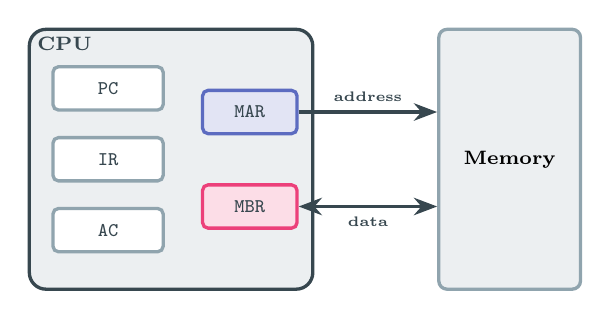
\begin{tikzpicture}[>=Stealth]
        \node[draw=nInk, very thick, rounded corners=6pt, fill=nFill, minimum width=3.6cm,
          minimum height=3.3cm] (cpu) at (0,0) {};
        \node[font=\scriptsize\bfseries, text=nInk, anchor=north west] at (cpu.north west) {CPU};
        \node[reg, minimum width=1.4cm] at (-0.8,0.9) {\textbf{PC}};
        \node[reg, minimum width=1.4cm] at (-0.8,0.0) {\textbf{IR}};
        \node[reg, minimum width=1.4cm] at (-0.8,-0.9) {\textbf{AC}};
        \node[reg, minimum width=1.2cm, fill=sIndigo!18, draw=sIndigo] (mar) at (1.0,0.6) {\textbf{MAR}};
        \node[reg, minimum width=1.2cm, fill=sPink!18, draw=sPink] (mbr) at (1.0,-0.6) {\textbf{MBR}};
        \node[dpmem, minimum width=1.8cm, minimum height=3.3cm] (mem) at (4.3,0) {Memory};
        \draw[-{Stealth}, very thick, nInk] (mar.east) -- node[above, font=\tiny\bfseries] {address}
          (mem.west |- mar.east);
        \draw[{Stealth}-{Stealth}, very thick, nInk] (mbr.east) -- node[below, font=\tiny\bfseries] {data}
          (mem.west |- mbr.east);
      \end{tikzpicture}
    \column{0.42\textwidth}
      \defbox{\textbf{MAR} (Memory Address Register) holds the \textbf{address} the CPU sends to memory.}
      \defbox{\textbf{MBR} (Memory Buffer Register) holds the \textbf{value} coming from memory
        or going to memory.}
      \stepbox{Like a post office counter}{you give the box number (MAR) and receive the parcel (MBR).}
  \end{columns}
  \vfill
  \keymsg{You can see both registers in MARIE.js, next to PC, IR and AC.}
\end{frame}

\begin{frame}{The bus: one road for everyone}
  \begin{center}
    \resizebox{0.8\textwidth}{!}{\busdiagram{none}{none}{}}
  \end{center}
  \vspace{0.1cm}
  \begin{columns}[T,onlytextwidth]
    \column{0.48\textwidth}
      \stepbox{The bus}{MARIE connects its registers and the memory with \textbf{one shared bus}.
        Values travel between them along this bus.}
    \column{0.48\textwidth}
      \stepbox{One value at a time}{At any moment the bus can carry \textbf{only one value}.
        The ALU has its own direct connections to the AC and the MBR.}
  \end{columns}
  \vfill
  \keymsg{So moving data takes \textbf{several steps}, one after another. One step is one \textbf{micro-operation},
    e.g.\ \mo{MAR}{PC}. We number the steps T0, T1, T2, \dots}
\end{frame}

\begin{frame}{Read and Write: how the control unit drives the bus}
  \begin{center}
    \resizebox{0.72\textwidth}{!}{\busdiagram{pc}{mar}{}}\\[0.02cm]
    \dplegend
  \end{center}
  \vspace{-0.1cm}
  \begin{columns}[T,onlytextwidth]
    \column{0.48\textwidth}
      \stepbox{\textcolor{ReadBlue}{Read}}{The control unit tells one element: ``put your value on the bus''.
        It is marked \textcolor{ReadBlue}{\textbf{blue}}.}
    \column{0.48\textwidth}
      \stepbox{\textcolor{WriteRed}{Write}}{The control unit tells one element: ``store the value from the bus''.
        It is marked \textcolor{WriteRed}{\textbf{red}}.}
  \end{columns}
  \vfill
  \keymsg{In a micro-operation $X \leftarrow Y$: \ $Y$ gets \textcolor{ReadBlue}{\textbf{Read}}, \ $X$ gets \textcolor{WriteRed}{\textbf{Write}}.
    Example above: \mo{MAR}{PC}.}
\end{frame}

\begin{frame}[fragile]{The program we will follow}
  \begin{columns}[c,onlytextwidth]
    \column{0.36\textwidth}
      \footnotesize\textbf{Exercise 1 from Day 1}
\begin{lstlisting}[style=marie]
Load X
Add Y
Store Z
Halt
X, DEC 5
Y, DEC 3
Z, DEC 0
\end{lstlisting}
    \column{0.6\textwidth}
      \centering\footnotesize\textbf{Memory after assembling}\\[0.1cm]
      \scriptsize
      \renewcommand{\arraystretch}{1.2}
      \begin{tabular}{ccll}
        \toprule
        \textbf{Address} & \textbf{Contents} & \textbf{Meaning} & \\
        \midrule
        \rowcolor{AccentOrange!15} 0 & \texttt{1004} & \texttt{Load X} & $\leftarrow$ we follow this one \\
        1 & \texttt{3005} & \texttt{Add Y} & \\
        2 & \texttt{2006} & \texttt{Store Z} & \\
        3 & \texttt{7000} & \texttt{Halt} & \\
        4 & \texttt{0005} & \texttt{X} = 5 & \\
        5 & \texttt{0003} & \texttt{Y} = 3 & \\
        6 & \texttt{0000} & \texttt{Z} = 0 & \\
        \bottomrule
      \end{tabular}
  \end{columns}
  \vfill
  \keymsg{We follow the first instruction, \texttt{Load X}, step by step.
    In MARIE.js you can watch the same steps with the \textbf{Micro step} button:
    the \textbf{Step} dots in the control unit show T0, T1, T2, \dots}
\end{frame}

% ---------- Fetch, step by step ----------
\stepframe{Fetch, step T0: \mo{MAR}{PC}}{pc}{mar}{step=0, mem=1004}
  {\stepbox{T0}{The PC puts the address of the next instruction (\textbf{0}) on the bus, and the MAR stores it.
     The memory now knows \textbf{which cell} the CPU wants.}
   \phasename{fetch}}

\stepframe{Fetch, step T1: \mo{MBR}{M[MAR]}}{mem}{mbr}{step=1, mem=1004, mbr=1004}
  {\stepbox{T1}{The memory returns the contents of cell 0: \texttt{1004} (\texttt{Load X}).
     The instruction waits in the MBR.}
   \phasename{fetch}}

\stepframe{Fetch, step T2: \mo{IR}{MBR}}{mbr}{ir}{step=2, mem=1004, mbr=1004, ir=1004}
  {\stepbox{T2}{The instruction moves from the MBR into the IR.}
   \phasename{fetch}}

\stepframe{Fetch, step T3: \mo{PC}{PC + 1}}{none}{pc}{step=3, mem=1004, mbr=1004, ir=1004, pc=001}
  {\stepbox{T3}{The PC is increased by 1. It already points to the next instruction.}
   \phasename{fetch}\vspace{0.06cm}
   \begin{beamercolorbox}[rounded=true,sep=0.08cm,wd=\linewidth]{block body example}
     \footnotesize\centering Day 1: \ $\mathsf{IR}\leftarrow\mathsf{M}[\mathsf{PC}]$, \ $\mathsf{PC}\leftarrow\mathsf{PC}+1$.
     \ In reality: \textbf{4 steps}.
   \end{beamercolorbox}}

% ---------- Execute Load X ----------
\stepframe{Execute \texttt{Load X}, step T4: \mo{MAR}{IR[11-0]}}{ir}{mar}{step=4, mem=0005, mbr=1004, ir=1004, pc=001, mar=004}
  {\stepbox{T4}{The address part of the instruction (\textbf{4}, the address of \texttt{X}) goes into the MAR.
     \texttt{IR[11-0]} means bits 11 to 0 of the IR: the address field.}
   \phasename{execute}}

\stepframe{Execute \texttt{Load X}, step T5: \mo{MBR}{M[MAR]}}{mem}{mbr}{step=5, mem=0005, mbr=0005, ir=1004, pc=001, mar=004}
  {\stepbox{T5}{The memory returns the contents of cell 4: \textbf{5}. The value waits in the MBR.}
   \phasename{execute}}

\stepframe{Execute \texttt{Load X}, step T6: \mo{AC}{MBR}}{mbr}{ac}{step=6, mem=0005, mbr=0005, ir=1004, pc=001, mar=004, ac=0005}
  {\stepbox{T6}{The value moves from the MBR into the AC.}
   \phasename{execute}\vspace{0.06cm}
   \begin{beamercolorbox}[rounded=true,sep=0.1cm,wd=\linewidth]{block body example}
     \footnotesize\centering Same result as on Day 1, now step by step.
   \end{beamercolorbox}}

\begin{frame}{How long does one instruction take?}
  \begin{center}
    
\begin{tikzpicture}[scale=1.25, every node/.style={transform shape}]
      \foreach \i in {0,...,3}
        \node[draw=white, fill=sAmber, text=black, font=\tiny\bfseries, minimum width=0.62cm,
          minimum height=0.45cm, inner sep=0pt] at ({0.62*\i},0) {T\i};
      \node[draw=white, fill=sBrown, text=white, font=\tiny\bfseries, minimum width=0.62cm,
        minimum height=0.45cm, inner sep=0pt] at ({0.62*4},0) {dec.};
      \foreach \i in {4,...,6}
        \node[draw=white, fill=sTeal, text=white, font=\tiny\bfseries, minimum width=0.62cm,
          minimum height=0.45cm, inner sep=0pt] at ({0.62*(\i+1)},0) {T\i};
      \node[anchor=west, font=\scriptsize] at ({0.62*8-0.25},0) {\texttt{Load} = 4 + 3 = \textbf{7 steps}};
    \end{tikzpicture}\\[0.05cm]
    {\tiny\textcolor{sAmber}{\rule{0.25cm}{0.2cm}}\ fetch
    \qquad\textcolor{sBrown}{\rule{0.25cm}{0.2cm}}\ decode
    \qquad\textcolor{sTeal}{\rule{0.25cm}{0.2cm}}\ execute}
  \end{center}
  \vspace{-0.15cm}
  \begin{center}
    \scriptsize
    \renewcommand{\arraystretch}{1.0}
    \begin{tabular}{cll}
      \toprule
      \textbf{Step} & \textbf{Micro-operation} & \textbf{Phase} \\
      \midrule
      T0 & \mo{MAR}{PC} & fetch \\
      T1 & \mo{MBR}{M[MAR]} & fetch \\
      T2 & \mo{IR}{MBR} & fetch \\
      T3 & \mo{PC}{PC + 1} & fetch \\
      -- & the CU decodes the opcode in \texttt{IR[15-12]} & decode \\
      T4 & \mo{MAR}{IR[11-0]} & execute \\
      T5 & \mo{MBR}{M[MAR]} & execute \\
      T6 & \mo{AC}{MBR} & execute \\
      \bottomrule
    \end{tabular}
  \end{center}
  \vspace{-0.1cm}
  \begin{columns}[T,onlytextwidth]
    \column{0.24\textwidth}
      \stepbox{Fetch}{is the \textbf{same} for every instruction.}
    \column{0.36\textwidth}
      \stepbox{Decode}{moves no data. The decoder works out the opcode while the PC is being increased,
        so in MARIE it needs no step of its own.}
    \column{0.36\textwidth}
      \stepbox{Execute}{depends on the instruction. E.g.\ \texttt{LoadI} needs \textbf{9 steps},
        because it reads the memory twice to get its value.}
  \end{columns}
\end{frame}

\begin{frame}[fragile]{Exercise 3: count the control signals}
  \begin{columns}[T,onlytextwidth]
    \column{0.33\textwidth}
\begin{lstlisting}[style=marie]
Load X
Add Y
Store Z
Output
Jump Stop
Stop, Halt
X, DEC 5
Y, DEC 3
Z, DEC 0
\end{lstlisting}
    \column{0.64\textwidth}
      \taskhead{Task}{Press \textbf{Assemble}, turn on \textbf{Data Path} and use \textbf{Micro step}.}
      \footnotesize
      \begin{enumerate}\setlength{\itemsep}{4pt}
        \item Choose one instruction: \texttt{Add Y}, \texttt{Store Z}, \texttt{Output} or \texttt{Jump Stop}.
        \item Go through it step by step, \textbf{including its fetch}. Count how many times the control unit
          sends a \textcolor{ReadBlue}{\textbf{Read}} signal and how many times a \textcolor{WriteRed}{\textbf{Write}} signal.
        \item In which step is there a Write but no Read? Why?
      \end{enumerate}
      \vspace{0.05cm}
      \begin{beamercolorbox}[rounded=true,sep=0.1cm,wd=\linewidth]{block body}
        \scriptsize\textbf{Hint:} in a micro-operation $X \leftarrow Y$, \ $Y$ is marked
        \textcolor{ReadBlue}{\textbf{blue}} (Read: it puts its value on the bus) and $X$ is marked
        \textcolor{WriteRed}{\textbf{red}} (Write: it stores the value).
        The Step dots show the current step; Micro step also stops once for the decode.
      \end{beamercolorbox}
  \end{columns}
\end{frame}

\begin{frame}{Solution: count the control signals}
  \begin{columns}[c,onlytextwidth]
    \column{0.55\textwidth}
      \centering
      \footnotesize\textbf{Questions 1 and 2}\\[0.1cm]
      \scriptsize
      \renewcommand{\arraystretch}{1.25}
      \begin{tabular}{lccc}
        \toprule
        & \textcolor{ReadBlue}{\textbf{Read}} & \textcolor{WriteRed}{\textbf{Write}} & \textbf{Steps} \\
        \midrule
        Fetch (the same for all) & 3 & 4 & 4 \\
        \midrule
        \texttt{Add Y}: fetch + 3 steps & 6 & 7 & 7 \\
        \texttt{Store Z}: fetch + 3 steps & 6 & 7 & 7 \\
        \texttt{Output}: fetch + \mo{OUT}{AC} & 4 & 5 & 5 \\
        \texttt{Jump Stop}: fetch + \mo{PC}{IR[11-0]} & 4 & 5 & 5 \\
        \bottomrule
      \end{tabular}
    \column{0.42\textwidth}
      \stepbox{Question 3}{In \mo{PC}{PC + 1}. Nothing travels on the bus: the PC increases itself.
        So there is a Write to the PC, but no Read.}
      \stepbox{Notice}{\textbf{Every step has a Write}: each micro-operation changes exactly one element.
        Instructions that use the memory need more steps.}
  \end{columns}
  \vfill
  \keymsg{\textbf{Read} and \textbf{Write} are signals from the control unit: it switches them on in the right step.
    More about this in Part 3.}
\end{frame}

% ---------- NEW: the von Neumann bottleneck and the Harvard architecture ----------
\newcommand{\diagVN}{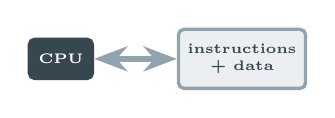
\begin{tikzpicture}[>=Stealth]
  \node[draw=nInk, very thick, fill=nInk, text=white, rounded corners=2pt, font=\tiny\bfseries,
    minimum width=0.8cm, minimum height=0.5cm] (c) at (0,0) {CPU};
  \node[draw=nLine, very thick, fill=nFill, text=nInk, rounded corners=2pt, font=\tiny\bfseries, align=center,
    minimum width=1.5cm, minimum height=0.75cm] (m) at (2.3,0) {instructions\\+ data};
  \draw[<->, line width=2pt, nLine] (c) -- (m);
\end{tikzpicture}}
\newcommand{\diagHarv}{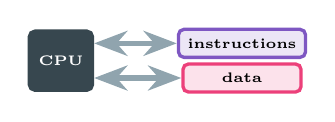
\begin{tikzpicture}[>=Stealth]
  \node[draw=nInk, very thick, fill=nInk, text=white, rounded corners=2pt, font=\tiny\bfseries,
    minimum width=0.8cm, minimum height=0.75cm] (c) at (0,0) {CPU};
  \node[draw=sViolet, very thick, fill=sViolet!15, rounded corners=2pt, font=\tiny\bfseries,
    minimum width=1.5cm, minimum height=0.33cm] (i) at (2.3,0.22) {instructions};
  \node[draw=sPink, very thick, fill=sPink!15, rounded corners=2pt, font=\tiny\bfseries,
    minimum width=1.5cm, minimum height=0.33cm] (d) at (2.3,-0.22) {data};
  \draw[<->, line width=2pt, nLine] (c.east |- i) -- (i);
  \draw[<->, line width=2pt, nLine] (c.east |- d) -- (d);
\end{tikzpicture}}
\newcommand{\diagModHarv}{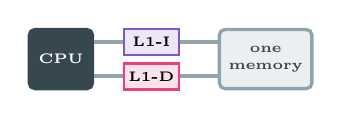
\begin{tikzpicture}[>=Stealth]
  \node[draw=nInk, very thick, fill=nInk, text=white, rounded corners=2pt, font=\tiny\bfseries,
    minimum width=0.8cm, minimum height=0.75cm] (c) at (0,0) {CPU};
  \node[draw=sViolet, thick, fill=sViolet!15, font=\tiny\bfseries, minimum width=0.7cm,
    minimum height=0.33cm, inner sep=1pt] (i) at (1.15,0.22) {L1-I};
  \node[draw=sPink, thick, fill=sPink!15, font=\tiny\bfseries, minimum width=0.7cm,
    minimum height=0.33cm, inner sep=1pt] (d) at (1.15,-0.22) {L1-D};
  \node[draw=nLine, very thick, fill=nFill, text=nInk, rounded corners=2pt, font=\tiny\bfseries, align=center,
    minimum width=1.0cm, minimum height=0.75cm] (m) at (2.6,0) {one\\memory};
  \draw[line width=1.5pt, nLine] (c.east |- i) -- (i);
  \draw[line width=1.5pt, nLine] (c.east |- d) -- (d);
  \draw[line width=1.5pt, nLine] (i.east) -- (m.west |- i);
  \draw[line width=1.5pt, nLine] (d.east) -- (m.west |- d);
\end{tikzpicture}}

\begin{frame}{One bus for everything: the von Neumann bottleneck}
  \begin{beamercolorbox}[rounded=true,sep=0.1cm,wd=\textwidth]{block body}
    \centering\footnotesize In Exercise 3, \textbf{4 of the 7 steps} of \texttt{Add Y} were the fetch.
    Instructions and data travel on the \textbf{same bus} to the \textbf{same memory}, so they must take turns.
  \end{beamercolorbox}
  \vspace{0.15cm}
  \begin{columns}[T,onlytextwidth]
    \column{0.31\textwidth}
      \optcard{Von Neumann (MARIE)}{\diagVN}
        {one memory: programs and data share the space (Day 1, Decision 2)}
        {the CPU cannot fetch an instruction and read data \textbf{at the same time}}
    \column{0.31\textwidth}
      \optcard{Harvard}{\diagHarv}
        {two separate roads: fetch and data \textbf{at the same time}}
        {two memories: ``address 0 exists twice'', and the space cannot be shared}
    \column{0.31\textwidth}
      \optcard{Modified Harvard (today)}{\diagModHarv}
        {separate roads \textbf{near} the CPU, but still one main memory}
        {more hardware: small copies (cache) that must be kept up to date}
  \end{columns}
  \vfill
  \keymsg{Today's processors are \textbf{Harvard close to the CPU} and \textbf{von Neumann further away}:
    the modified Harvard architecture. We will meet the L1 cache again later.}
\end{frame}

% =====================================================================
\section{The control unit}
% =====================================================================

\begin{frame}{Who flips all the switches?}
  \begin{columns}[c,onlytextwidth]
    \column{0.45\textwidth}
      \begin{beamercolorbox}[rounded=true,sep=0.12cm,wd=\linewidth]{block body}
        \centering\small
        Day 1: the \textbf{CU} decides and coordinates, but never calculates.
      \end{beamercolorbox}
      \vspace{0.2cm}
      \begin{beamercolorbox}[rounded=true,sep=0.12cm,wd=\linewidth]{block body}
        \centering\small
        Today: an instruction is a sequence of micro-operations, one per step.
      \end{beamercolorbox}
    \column{0.5\textwidth}
      \centering
      
\begin{tikzpicture}
        \node[cpuunit, draw=nLine, fill=nFill, minimum width=2.2cm, minimum height=1.2cm,
          font=\large\bfseries, text=nInk] (cu) {CU};
        \node[font=\Huge\bfseries, text=AccentOrange, right=0.4cm of cu] {?};
      \end{tikzpicture}
  \end{columns}
  \vfill
  \begin{alertblock}{The question}
    \small How does the CU know \textbf{what to switch on} in each step?
  \end{alertblock}
\end{frame}

\begin{frame}{How the CU decides: card and row}
  \vfill
  \begin{center}
    \resizebox{\textwidth}{!}{%
    \begin{tikzpicture}[>=Stealth]
    \fill[white] (3.6,3.25) rectangle (7.0,1.47);
    \fill[nLight] (3.6,3.25) rectangle (7.0,2.91);
    \node[font=\tiny\bfseries, text=black] at (5.300,3.080) {Fetch (every instruction)};
    \node[font=\tiny, text=black!45, anchor=west] at (3.680,2.790) {Step};
    \node[font=\tiny, text=ReadBlue, anchor=west] at (4.100,2.790) {Read};
    \node[font=\tiny, text=WriteRed, anchor=west] at (5.550,2.790) {Write};
    \node[font=\tiny\bfseries, text=black, anchor=west] at (3.680,2.520) {T0};
    \node[font=\ttfamily\tiny, text=black, anchor=west] at (4.100,2.520) {PC};
    \node[font=\ttfamily\tiny, text=black, anchor=west] at (5.550,2.520) {MAR};
    \node[font=\tiny\bfseries, text=black, anchor=west] at (3.680,2.220) {T1};
    \node[font=\ttfamily\tiny, text=black, anchor=west] at (4.100,2.220) {memory};
    \node[font=\ttfamily\tiny, text=black, anchor=west] at (5.550,2.220) {MBR};
    \node[font=\tiny\bfseries, text=black, anchor=west] at (3.680,1.920) {T2};
    \node[font=\ttfamily\tiny, text=black, anchor=west] at (4.100,1.920) {MBR};
    \node[font=\ttfamily\tiny, text=black, anchor=west] at (5.550,1.920) {IR};
    \node[font=\tiny\bfseries, text=black, anchor=west] at (3.680,1.620) {T3};
    \node[font=\ttfamily\tiny, text=black, anchor=west] at (4.100,1.620) {--};
    \node[font=\ttfamily\tiny, text=black, anchor=west] at (5.550,1.620) {PC +1};
    \draw[nLine, line width=1.3pt, rounded corners=2pt] (3.6,3.25) rectangle (7.0,1.47);
    \node[font=\tiny, text width=2.6cm, align=left, anchor=north west, text=black!70] at (7.15,3.25) {The same for every instruction: before the decode, the CU does not know the opcode yet.};
    \node[draw=nLight, fill=LightGray, rounded corners=2pt, anchor=north east, inner sep=3pt, font=\tiny] at (14.05,3.25) {%
  \begin{tabular}{@{}cl@{}}\multicolumn{2}{@{}l}{\textbf{Reminder: opcodes}}\\[1pt]
  \texttt{1} & \texttt{Load X}\\ \texttt{2} & \texttt{Store X}\\ \texttt{3} & \texttt{Add X}\\ \texttt{9} & \texttt{Jump X}\end{tabular}};
    \only<1>{\node[draw=nLine, thick, fill=sViolet!20, minimum width=0.6cm, minimum height=0.45cm, font=\ttfamily\scriptsize] (op) at (0.55,2.4) {1};
    \node[draw=nLine, thick, fill=white, minimum width=1.2cm, minimum height=0.45cm, font=\ttfamily\scriptsize, right=0pt of op] (ad) {004};}
    \only<2>{\node[draw=nLine, thick, fill=sViolet!20, minimum width=0.6cm, minimum height=0.45cm, font=\ttfamily\scriptsize] (op) at (0.55,2.4) {2};
    \node[draw=nLine, thick, fill=white, minimum width=1.2cm, minimum height=0.45cm, font=\ttfamily\scriptsize, right=0pt of op] (ad) {006};}
    \only<3>{\node[draw=nLine, thick, fill=sViolet!20, minimum width=0.6cm, minimum height=0.45cm, font=\ttfamily\scriptsize] (op) at (0.55,2.4) {9};
    \node[draw=nLine, thick, fill=white, minimum width=1.2cm, minimum height=0.45cm, font=\ttfamily\scriptsize, right=0pt of op] (ad) {005};}
    \node[font=\tiny, text=nLine] at (1.15,2.78) {IR};
    \node[font=\tiny, text=sViolet] at (0.55,2.02) {opcode};
    \node[draw=nLine, thick, fill=LightGray, minimum width=2.2cm, minimum height=1.1cm] (cu) at (1.2,0.2) {};
    \node[font=\scriptsize\bfseries, text=nInk] at (1.2,0.45) {Control unit};
    \only<1>{\node[font=\scriptsize] at (1.2,0.05) {Step: \textbf{T5}};}
    \only<2>{\node[font=\scriptsize] at (1.2,0.05) {Step: \textbf{T5}};}
    \only<3>{\node[font=\scriptsize] at (1.2,0.05) {Step: \textbf{T4}};}
    \draw[thick, nInk, -{Stealth[length=2mm, width=1.8mm]}] (0.55,1.88) -- (0.55,0.77);
    \draw[line width=1.1pt, nInk, -{Stealth[length=2.2mm, width=2mm]}, shorten >= 2pt, rounded corners=2pt] (2.3,0.55) -- (2.8,0.55) -- (2.8,2.2) -- (3.58,2.2);
    \node[circle, fill=AccentOrange, text=white, font=\tiny\bfseries, inner sep=1pt] at (2.8,1.35) {1};
    \node[font=\tiny, text=nInk, anchor=south] at (3.2,2.22) {first};
    \only<1>{\fill[white] (3.6,1.0) rectangle (6.1,-0.48);
  \fill[AccentOrange!20] (3.6,1.0) rectangle (6.1,0.66);
  \node[font=\tiny\bfseries, text=black] at (4.850,0.830) {\texttt{Load} (opcode 1)};
  \node[font=\tiny, text=black!45, anchor=west] at (3.680,0.540) {Step};
  \node[font=\tiny, text=ReadBlue, anchor=west] at (4.100,0.540) {Read};
  \node[font=\tiny, text=WriteRed, anchor=west] at (5.100,0.540) {Write};
  \node[font=\tiny\bfseries, text=black, anchor=west] at (3.680,0.270) {T4};
  \node[font=\ttfamily\tiny, text=black, anchor=west] at (4.100,0.270) {IR};
  \node[font=\ttfamily\tiny, text=black, anchor=west] at (5.100,0.270) {MAR};
  \fill[AccentOrange!22] (3.6,0.120) rectangle (6.1,-0.180);
  \node[font=\tiny\bfseries, text=black, anchor=west] at (3.680,-0.030) {T5};
  \node[font=\ttfamily\tiny, text=black, anchor=west] at (4.100,-0.030) {memory};
  \node[font=\ttfamily\tiny, text=black, anchor=west] at (5.100,-0.030) {MBR};
  \node[font=\tiny\bfseries, text=black, anchor=west] at (3.680,-0.330) {T6};
  \node[font=\ttfamily\tiny, text=black, anchor=west] at (4.100,-0.330) {MBR};
  \node[font=\ttfamily\tiny, text=black, anchor=west] at (5.100,-0.330) {AC};
  \draw[AccentOrange, line width=1.3pt, rounded corners=2pt] (3.6,1.0) rectangle (6.1,-0.48);
  \fill[white] (6.25,1.0) rectangle (8.75,-0.48);
  \fill[LightGray] (6.25,1.0) rectangle (8.75,0.66);
  \node[font=\tiny\bfseries, text=black!35] at (7.500,0.830) {\texttt{Store} (opcode 2)};
  \node[font=\tiny, text=black!45, anchor=west] at (6.330,0.540) {Step};
  \node[font=\tiny, text=black!35, anchor=west] at (6.750,0.540) {Read};
  \node[font=\tiny, text=black!35, anchor=west] at (7.750,0.540) {Write};
  \node[font=\tiny\bfseries, text=black!35, anchor=west] at (6.330,0.270) {T4};
  \node[font=\ttfamily\tiny, text=black!35, anchor=west] at (6.750,0.270) {IR};
  \node[font=\ttfamily\tiny, text=black!35, anchor=west] at (7.750,0.270) {MAR};
  \node[font=\tiny\bfseries, text=black!35, anchor=west] at (6.330,-0.030) {T5};
  \node[font=\ttfamily\tiny, text=black!35, anchor=west] at (6.750,-0.030) {AC};
  \node[font=\ttfamily\tiny, text=black!35, anchor=west] at (7.750,-0.030) {MBR};
  \node[font=\tiny\bfseries, text=black!35, anchor=west] at (6.330,-0.330) {T6};
  \node[font=\ttfamily\tiny, text=black!35, anchor=west] at (6.750,-0.330) {MBR};
  \node[font=\ttfamily\tiny, text=black!35, anchor=west] at (7.750,-0.330) {memory};
  \draw[nLight, thick, rounded corners=2pt] (6.25,1.0) rectangle (8.75,-0.48);
  \fill[white] (8.9,1.0) rectangle (11.4,-0.48);
  \fill[LightGray] (8.9,1.0) rectangle (11.4,0.66);
  \node[font=\tiny\bfseries, text=black!35] at (10.150,0.830) {\texttt{Add} (opcode 3)};
  \node[font=\tiny, text=black!45, anchor=west] at (8.980,0.540) {Step};
  \node[font=\tiny, text=black!35, anchor=west] at (9.400,0.540) {Read};
  \node[font=\tiny, text=black!35, anchor=west] at (10.400,0.540) {Write};
  \node[font=\tiny\bfseries, text=black!35, anchor=west] at (8.980,0.270) {T4};
  \node[font=\ttfamily\tiny, text=black!35, anchor=west] at (9.400,0.270) {IR};
  \node[font=\ttfamily\tiny, text=black!35, anchor=west] at (10.400,0.270) {MAR};
  \node[font=\tiny\bfseries, text=black!35, anchor=west] at (8.980,-0.030) {T5};
  \node[font=\ttfamily\tiny, text=black!35, anchor=west] at (9.400,-0.030) {memory};
  \node[font=\ttfamily\tiny, text=black!35, anchor=west] at (10.400,-0.030) {MBR};
  \node[font=\tiny\bfseries, text=black!35, anchor=west] at (8.980,-0.330) {T6};
  \node[font=\ttfamily\tiny, text=black!35, anchor=west] at (9.400,-0.330) {MBR};
  \node[font=\ttfamily\tiny, text=black!35, anchor=west] at (10.400,-0.330) {AC \scalebox{0.8}{(add)}};
  \draw[nLight, thick, rounded corners=2pt] (8.9,1.0) rectangle (11.4,-0.48);
  \fill[white] (11.55,1.0) rectangle (14.05,0.12);
  \fill[LightGray] (11.55,1.0) rectangle (14.05,0.66);
  \node[font=\tiny\bfseries, text=black!35] at (12.800,0.830) {\texttt{Jump} (opcode 9)};
  \node[font=\tiny, text=black!45, anchor=west] at (11.630,0.540) {Step};
  \node[font=\tiny, text=black!35, anchor=west] at (12.050,0.540) {Read};
  \node[font=\tiny, text=black!35, anchor=west] at (13.050,0.540) {Write};
  \node[font=\tiny\bfseries, text=black!35, anchor=west] at (11.630,0.270) {T4};
  \node[font=\ttfamily\tiny, text=black!35, anchor=west] at (12.050,0.270) {IR};
  \node[font=\ttfamily\tiny, text=black!35, anchor=west] at (13.050,0.270) {PC};
  \draw[nLight, thick, rounded corners=2pt] (11.55,1.0) rectangle (14.05,0.12);
  \draw[line width=1.1pt, nInk, -{Stealth[length=2.2mm, width=2mm]}, shorten >= 2pt, rounded corners=2pt] (2.3,-0.030) -- (3.580,-0.030);
  \node[circle, fill=AccentOrange, text=white, font=\tiny\bfseries, inner sep=1pt] at (2.95,-0.030) {2};
  \node[font=\tiny, text=nInk, anchor=north west] at (2.7,-0.88) {then: the opcode picks the card, the step picks the row};}
    \only<2>{\fill[white] (3.6,1.0) rectangle (6.1,-0.48);
  \fill[LightGray] (3.6,1.0) rectangle (6.1,0.66);
  \node[font=\tiny\bfseries, text=black!35] at (4.850,0.830) {\texttt{Load} (opcode 1)};
  \node[font=\tiny, text=black!45, anchor=west] at (3.680,0.540) {Step};
  \node[font=\tiny, text=black!35, anchor=west] at (4.100,0.540) {Read};
  \node[font=\tiny, text=black!35, anchor=west] at (5.100,0.540) {Write};
  \node[font=\tiny\bfseries, text=black!35, anchor=west] at (3.680,0.270) {T4};
  \node[font=\ttfamily\tiny, text=black!35, anchor=west] at (4.100,0.270) {IR};
  \node[font=\ttfamily\tiny, text=black!35, anchor=west] at (5.100,0.270) {MAR};
  \node[font=\tiny\bfseries, text=black!35, anchor=west] at (3.680,-0.030) {T5};
  \node[font=\ttfamily\tiny, text=black!35, anchor=west] at (4.100,-0.030) {memory};
  \node[font=\ttfamily\tiny, text=black!35, anchor=west] at (5.100,-0.030) {MBR};
  \node[font=\tiny\bfseries, text=black!35, anchor=west] at (3.680,-0.330) {T6};
  \node[font=\ttfamily\tiny, text=black!35, anchor=west] at (4.100,-0.330) {MBR};
  \node[font=\ttfamily\tiny, text=black!35, anchor=west] at (5.100,-0.330) {AC};
  \draw[nLight, thick, rounded corners=2pt] (3.6,1.0) rectangle (6.1,-0.48);
  \fill[white] (6.25,1.0) rectangle (8.75,-0.48);
  \fill[AccentOrange!20] (6.25,1.0) rectangle (8.75,0.66);
  \node[font=\tiny\bfseries, text=black] at (7.500,0.830) {\texttt{Store} (opcode 2)};
  \node[font=\tiny, text=black!45, anchor=west] at (6.330,0.540) {Step};
  \node[font=\tiny, text=ReadBlue, anchor=west] at (6.750,0.540) {Read};
  \node[font=\tiny, text=WriteRed, anchor=west] at (7.750,0.540) {Write};
  \node[font=\tiny\bfseries, text=black, anchor=west] at (6.330,0.270) {T4};
  \node[font=\ttfamily\tiny, text=black, anchor=west] at (6.750,0.270) {IR};
  \node[font=\ttfamily\tiny, text=black, anchor=west] at (7.750,0.270) {MAR};
  \fill[AccentOrange!22] (6.25,0.120) rectangle (8.75,-0.180);
  \node[font=\tiny\bfseries, text=black, anchor=west] at (6.330,-0.030) {T5};
  \node[font=\ttfamily\tiny, text=black, anchor=west] at (6.750,-0.030) {AC};
  \node[font=\ttfamily\tiny, text=black, anchor=west] at (7.750,-0.030) {MBR};
  \node[font=\tiny\bfseries, text=black, anchor=west] at (6.330,-0.330) {T6};
  \node[font=\ttfamily\tiny, text=black, anchor=west] at (6.750,-0.330) {MBR};
  \node[font=\ttfamily\tiny, text=black, anchor=west] at (7.750,-0.330) {memory};
  \draw[AccentOrange, line width=1.3pt, rounded corners=2pt] (6.25,1.0) rectangle (8.75,-0.48);
  \fill[white] (8.9,1.0) rectangle (11.4,-0.48);
  \fill[LightGray] (8.9,1.0) rectangle (11.4,0.66);
  \node[font=\tiny\bfseries, text=black!35] at (10.150,0.830) {\texttt{Add} (opcode 3)};
  \node[font=\tiny, text=black!45, anchor=west] at (8.980,0.540) {Step};
  \node[font=\tiny, text=black!35, anchor=west] at (9.400,0.540) {Read};
  \node[font=\tiny, text=black!35, anchor=west] at (10.400,0.540) {Write};
  \node[font=\tiny\bfseries, text=black!35, anchor=west] at (8.980,0.270) {T4};
  \node[font=\ttfamily\tiny, text=black!35, anchor=west] at (9.400,0.270) {IR};
  \node[font=\ttfamily\tiny, text=black!35, anchor=west] at (10.400,0.270) {MAR};
  \node[font=\tiny\bfseries, text=black!35, anchor=west] at (8.980,-0.030) {T5};
  \node[font=\ttfamily\tiny, text=black!35, anchor=west] at (9.400,-0.030) {memory};
  \node[font=\ttfamily\tiny, text=black!35, anchor=west] at (10.400,-0.030) {MBR};
  \node[font=\tiny\bfseries, text=black!35, anchor=west] at (8.980,-0.330) {T6};
  \node[font=\ttfamily\tiny, text=black!35, anchor=west] at (9.400,-0.330) {MBR};
  \node[font=\ttfamily\tiny, text=black!35, anchor=west] at (10.400,-0.330) {AC \scalebox{0.8}{(add)}};
  \draw[nLight, thick, rounded corners=2pt] (8.9,1.0) rectangle (11.4,-0.48);
  \fill[white] (11.55,1.0) rectangle (14.05,0.12);
  \fill[LightGray] (11.55,1.0) rectangle (14.05,0.66);
  \node[font=\tiny\bfseries, text=black!35] at (12.800,0.830) {\texttt{Jump} (opcode 9)};
  \node[font=\tiny, text=black!45, anchor=west] at (11.630,0.540) {Step};
  \node[font=\tiny, text=black!35, anchor=west] at (12.050,0.540) {Read};
  \node[font=\tiny, text=black!35, anchor=west] at (13.050,0.540) {Write};
  \node[font=\tiny\bfseries, text=black!35, anchor=west] at (11.630,0.270) {T4};
  \node[font=\ttfamily\tiny, text=black!35, anchor=west] at (12.050,0.270) {IR};
  \node[font=\ttfamily\tiny, text=black!35, anchor=west] at (13.050,0.270) {PC};
  \draw[nLight, thick, rounded corners=2pt] (11.55,1.0) rectangle (14.05,0.12);
  \draw[line width=1.1pt, nInk, -{Stealth[length=2.2mm, width=2mm]}, shorten >= 2pt, rounded corners=2pt] (2.3,-0.030) -- (6.230,-0.030);
  \node[circle, fill=AccentOrange, text=white, font=\tiny\bfseries, inner sep=1pt] at (2.95,-0.030) {2};
  \node[font=\tiny, text=nInk, anchor=north west] at (2.7,-0.88) {then: the opcode picks the card, the step picks the row};}
    \only<3>{\fill[white] (3.6,1.0) rectangle (6.1,-0.48);
  \fill[LightGray] (3.6,1.0) rectangle (6.1,0.66);
  \node[font=\tiny\bfseries, text=black!35] at (4.850,0.830) {\texttt{Load} (opcode 1)};
  \node[font=\tiny, text=black!45, anchor=west] at (3.680,0.540) {Step};
  \node[font=\tiny, text=black!35, anchor=west] at (4.100,0.540) {Read};
  \node[font=\tiny, text=black!35, anchor=west] at (5.100,0.540) {Write};
  \node[font=\tiny\bfseries, text=black!35, anchor=west] at (3.680,0.270) {T4};
  \node[font=\ttfamily\tiny, text=black!35, anchor=west] at (4.100,0.270) {IR};
  \node[font=\ttfamily\tiny, text=black!35, anchor=west] at (5.100,0.270) {MAR};
  \node[font=\tiny\bfseries, text=black!35, anchor=west] at (3.680,-0.030) {T5};
  \node[font=\ttfamily\tiny, text=black!35, anchor=west] at (4.100,-0.030) {memory};
  \node[font=\ttfamily\tiny, text=black!35, anchor=west] at (5.100,-0.030) {MBR};
  \node[font=\tiny\bfseries, text=black!35, anchor=west] at (3.680,-0.330) {T6};
  \node[font=\ttfamily\tiny, text=black!35, anchor=west] at (4.100,-0.330) {MBR};
  \node[font=\ttfamily\tiny, text=black!35, anchor=west] at (5.100,-0.330) {AC};
  \draw[nLight, thick, rounded corners=2pt] (3.6,1.0) rectangle (6.1,-0.48);
  \fill[white] (6.25,1.0) rectangle (8.75,-0.48);
  \fill[LightGray] (6.25,1.0) rectangle (8.75,0.66);
  \node[font=\tiny\bfseries, text=black!35] at (7.500,0.830) {\texttt{Store} (opcode 2)};
  \node[font=\tiny, text=black!45, anchor=west] at (6.330,0.540) {Step};
  \node[font=\tiny, text=black!35, anchor=west] at (6.750,0.540) {Read};
  \node[font=\tiny, text=black!35, anchor=west] at (7.750,0.540) {Write};
  \node[font=\tiny\bfseries, text=black!35, anchor=west] at (6.330,0.270) {T4};
  \node[font=\ttfamily\tiny, text=black!35, anchor=west] at (6.750,0.270) {IR};
  \node[font=\ttfamily\tiny, text=black!35, anchor=west] at (7.750,0.270) {MAR};
  \node[font=\tiny\bfseries, text=black!35, anchor=west] at (6.330,-0.030) {T5};
  \node[font=\ttfamily\tiny, text=black!35, anchor=west] at (6.750,-0.030) {AC};
  \node[font=\ttfamily\tiny, text=black!35, anchor=west] at (7.750,-0.030) {MBR};
  \node[font=\tiny\bfseries, text=black!35, anchor=west] at (6.330,-0.330) {T6};
  \node[font=\ttfamily\tiny, text=black!35, anchor=west] at (6.750,-0.330) {MBR};
  \node[font=\ttfamily\tiny, text=black!35, anchor=west] at (7.750,-0.330) {memory};
  \draw[nLight, thick, rounded corners=2pt] (6.25,1.0) rectangle (8.75,-0.48);
  \fill[white] (8.9,1.0) rectangle (11.4,-0.48);
  \fill[LightGray] (8.9,1.0) rectangle (11.4,0.66);
  \node[font=\tiny\bfseries, text=black!35] at (10.150,0.830) {\texttt{Add} (opcode 3)};
  \node[font=\tiny, text=black!45, anchor=west] at (8.980,0.540) {Step};
  \node[font=\tiny, text=black!35, anchor=west] at (9.400,0.540) {Read};
  \node[font=\tiny, text=black!35, anchor=west] at (10.400,0.540) {Write};
  \node[font=\tiny\bfseries, text=black!35, anchor=west] at (8.980,0.270) {T4};
  \node[font=\ttfamily\tiny, text=black!35, anchor=west] at (9.400,0.270) {IR};
  \node[font=\ttfamily\tiny, text=black!35, anchor=west] at (10.400,0.270) {MAR};
  \node[font=\tiny\bfseries, text=black!35, anchor=west] at (8.980,-0.030) {T5};
  \node[font=\ttfamily\tiny, text=black!35, anchor=west] at (9.400,-0.030) {memory};
  \node[font=\ttfamily\tiny, text=black!35, anchor=west] at (10.400,-0.030) {MBR};
  \node[font=\tiny\bfseries, text=black!35, anchor=west] at (8.980,-0.330) {T6};
  \node[font=\ttfamily\tiny, text=black!35, anchor=west] at (9.400,-0.330) {MBR};
  \node[font=\ttfamily\tiny, text=black!35, anchor=west] at (10.400,-0.330) {AC \scalebox{0.8}{(add)}};
  \draw[nLight, thick, rounded corners=2pt] (8.9,1.0) rectangle (11.4,-0.48);
  \fill[white] (11.55,1.0) rectangle (14.05,0.12);
  \fill[AccentOrange!20] (11.55,1.0) rectangle (14.05,0.66);
  \node[font=\tiny\bfseries, text=black] at (12.800,0.830) {\texttt{Jump} (opcode 9)};
  \node[font=\tiny, text=black!45, anchor=west] at (11.630,0.540) {Step};
  \node[font=\tiny, text=ReadBlue, anchor=west] at (12.050,0.540) {Read};
  \node[font=\tiny, text=WriteRed, anchor=west] at (13.050,0.540) {Write};
  \fill[AccentOrange!22] (11.55,0.420) rectangle (14.05,0.120);
  \node[font=\tiny\bfseries, text=black, anchor=west] at (11.630,0.270) {T4};
  \node[font=\ttfamily\tiny, text=black, anchor=west] at (12.050,0.270) {IR};
  \node[font=\ttfamily\tiny, text=black, anchor=west] at (13.050,0.270) {PC};
  \draw[AccentOrange, line width=1.3pt, rounded corners=2pt] (11.55,1.0) rectangle (14.05,0.12);
  \draw[line width=1.1pt, nInk, -{Stealth[length=2.2mm, width=2mm]}, shorten >= 2pt, rounded corners=2pt] (2.3,0.270) -- (11.530,0.270);
  \node[circle, fill=AccentOrange, text=white, font=\tiny\bfseries, inner sep=1pt] at (2.95,-0.030) {2};
  \node[font=\tiny, text=nInk, anchor=north west] at (2.7,-0.88) {then: the opcode picks the card, the step picks the row};}
    \end{tikzpicture}}
  \end{center}
  \vfill
\end{frame}

\begin{frame}{How can we build such a control unit?}
  \vfill
  \begin{center}
    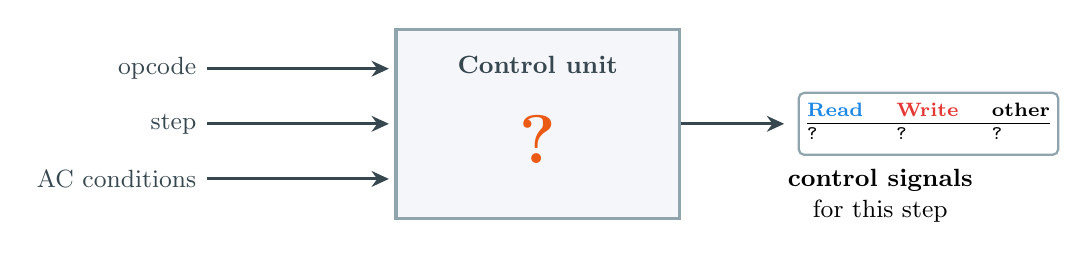
\begin{tikzpicture}[>=Stealth]
      \node[draw=nLine, very thick, fill=LightGray, minimum width=3.6cm, minimum height=2.4cm] (cu) at (0,0) {};
      \node[font=\small\bfseries, text=nInk] at (0,0.75) {Control unit};
      \node[font=\Huge\bfseries, text=AccentOrange] at (0,-0.2) {?};
      \foreach \y/\t in {0.7/opcode, 0/step, -0.7/{AC conditions}}
        \draw[line width=1.1pt, nInk, -{Stealth[length=2.2mm, width=2mm]}, shorten >= 2pt, rounded corners=2pt] (-4.2,\y) node[left, font=\small] {\t} -- (-1.82,\y);
      \draw[line width=1.1pt, nInk, -{Stealth[length=2.2mm, width=2mm]}, shorten >= 2pt, rounded corners=2pt] (1.82,0) -- (3.2,0);
      \node[anchor=west, draw=nLine, thick, fill=white, rounded corners=2pt, inner sep=3pt, font=\scriptsize] at (3.3,0) {%
        \begin{tabular}{@{}lll@{}}
          \textcolor{ReadBlue}{\textbf{Read}} & \textcolor{WriteRed}{\textbf{Write}} & \textbf{other} \\ \hline
          \texttt{?} & \texttt{?} & \texttt{?}
        \end{tabular}};
      \node[font=\small, anchor=north] at (4.35,-0.45) {\textbf{control signals}};
      \node[font=\small, anchor=north] at (4.35,-0.85) {for this step};
    \end{tikzpicture}
  \end{center}
  \vfill
\end{frame}

\begin{frame}{Way 1: hardwired control unit}
  \begin{columns}[c,onlytextwidth]
    \column{0.64\textwidth}
      \centering
      \resizebox{!}{5.5cm}{%
      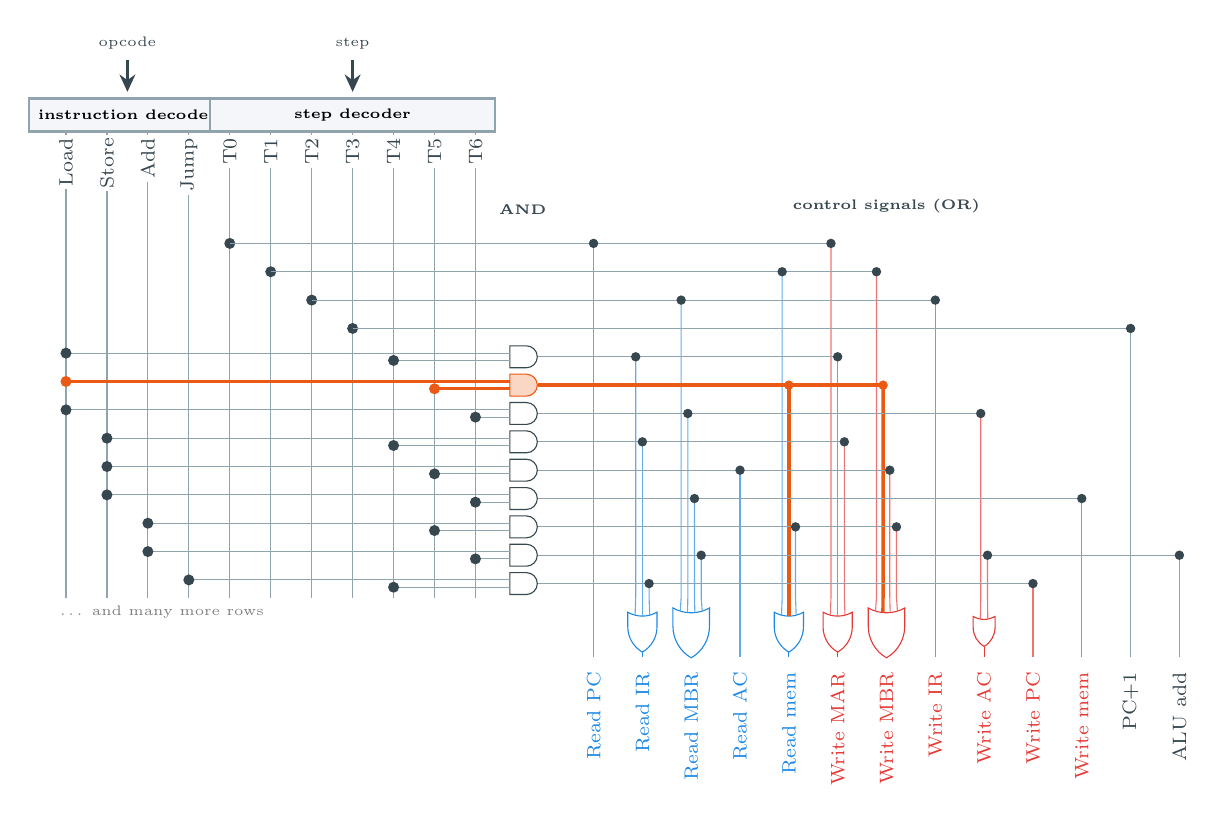
\begin{tikzpicture}[>=Stealth]
      \node[draw=nLine, thick, fill=LightGray, minimum height=0.42cm, minimum width=2.06cm, font=\tiny\bfseries] (idec) at (1.38,5.05) {instruction decoder};
      \node[draw=nLine, thick, fill=LightGray, minimum height=0.42cm, minimum width=3.62cm, font=\tiny\bfseries] (sdec) at (4.24,5.05) {step decoder};
      \draw[line width=1.1pt, nInk, -{Stealth[length=2.2mm, width=2mm]}, shorten >= 2pt, rounded corners=2pt] (1.38,5.75) node[above, font=\tiny] {opcode} -- (idec.north);
      \draw[line width=1.1pt, nInk, -{Stealth[length=2.2mm, width=2mm]}, shorten >= 2pt, rounded corners=2pt] (4.24,5.75) node[above, font=\tiny] {step} -- (sdec.north);
      \draw[nLine] (0.60,4.84) -- (0.60,-1.08);
      \node[font=\scriptsize, text=nInk, rotate=90, anchor=east, fill=white, inner sep=1pt] at (0.60,4.8) {Load};
      \draw[nLine] (1.12,4.84) -- (1.12,-1.08);
      \node[font=\scriptsize, text=nInk, rotate=90, anchor=east, fill=white, inner sep=1pt] at (1.12,4.8) {Store};
      \draw[nLine] (1.64,4.84) -- (1.64,-1.08);
      \node[font=\scriptsize, text=nInk, rotate=90, anchor=east, fill=white, inner sep=1pt] at (1.64,4.8) {Add};
      \draw[nLine] (2.16,4.84) -- (2.16,-1.08);
      \node[font=\scriptsize, text=nInk, rotate=90, anchor=east, fill=white, inner sep=1pt] at (2.16,4.8) {Jump};
      \draw[nLine] (2.68,4.84) -- (2.68,-1.08);
      \node[font=\scriptsize, text=nInk, rotate=90, anchor=east, fill=white, inner sep=1pt] at (2.68,4.8) {T0};
      \draw[nLine] (3.20,4.84) -- (3.20,-1.08);
      \node[font=\scriptsize, text=nInk, rotate=90, anchor=east, fill=white, inner sep=1pt] at (3.20,4.8) {T1};
      \draw[nLine] (3.72,4.84) -- (3.72,-1.08);
      \node[font=\scriptsize, text=nInk, rotate=90, anchor=east, fill=white, inner sep=1pt] at (3.72,4.8) {T2};
      \draw[nLine] (4.24,4.84) -- (4.24,-1.08);
      \node[font=\scriptsize, text=nInk, rotate=90, anchor=east, fill=white, inner sep=1pt] at (4.24,4.8) {T3};
      \draw[nLine] (4.76,4.84) -- (4.76,-1.08);
      \node[font=\scriptsize, text=nInk, rotate=90, anchor=east, fill=white, inner sep=1pt] at (4.76,4.8) {T4};
      \draw[nLine] (5.28,4.84) -- (5.28,-1.08);
      \node[font=\scriptsize, text=nInk, rotate=90, anchor=east, fill=white, inner sep=1pt] at (5.28,4.8) {T5};
      \draw[nLine] (5.80,4.84) -- (5.80,-1.08);
      \node[font=\scriptsize, text=nInk, rotate=90, anchor=east, fill=white, inner sep=1pt] at (5.80,4.8) {T6};
      \draw[ReadBlue!70] (7.300,3.42) -- (7.30,-1.83) coordinate (o0);
      \node[font=\scriptsize, text=ReadBlue, rotate=90, anchor=east] at (7.30,-1.90) {Read PC};
      \node[or gate US, draw=ReadBlue, fill=white, logic gate inputs=nnn, rotate=-90, scale=0.55] (or1) at (7.92,-1.48) {};
      \draw[ReadBlue!70] (7.835,1.98) -- (7.835,-1.08) -- (or1.input 3);
      \draw[ReadBlue!70] (7.920,0.90) -- (7.920,-1.08) -- (or1.input 2);
      \draw[ReadBlue!70] (8.005,-0.90) -- (8.005,-1.08) -- (or1.input 1);
      \draw[ReadBlue] (or1.output) -- (7.92,-1.83) coordinate (o1);
      \node[font=\scriptsize, text=ReadBlue, rotate=90, anchor=east] at (7.92,-1.90) {Read IR};
      \node[or gate US, draw=ReadBlue, fill=white, logic gate inputs=nnnn, rotate=-90, scale=0.55] (or2) at (8.54,-1.48) {};
      \draw[ReadBlue!70] (8.412,2.70) -- (8.412,-1.08) -- (or2.input 4);
      \draw[ReadBlue!70] (8.497,1.26) -- (8.497,-1.08) -- (or2.input 3);
      \draw[ReadBlue!70] (8.582,0.18) -- (8.582,-1.08) -- (or2.input 2);
      \draw[ReadBlue!70] (8.667,-0.54) -- (8.667,-1.08) -- (or2.input 1);
      \draw[ReadBlue] (or2.output) -- (8.54,-1.83) coordinate (o2);
      \node[font=\scriptsize, text=ReadBlue, rotate=90, anchor=east] at (8.54,-1.90) {Read MBR};
      \draw[ReadBlue!70] (9.160,0.54) -- (9.16,-1.83) coordinate (o3);
      \node[font=\scriptsize, text=ReadBlue, rotate=90, anchor=east] at (9.16,-1.90) {Read AC};
      \node[or gate US, draw=ReadBlue, fill=white, logic gate inputs=nnn, rotate=-90, scale=0.55] (or4) at (9.78,-1.48) {};
      \draw[ReadBlue!70] (9.695,3.06) -- (9.695,-1.08) -- (or4.input 3);
      \draw[AccentOrange, line width=1.2pt] (9.780,1.62) -- (9.780,-1.08) -- (or4.input 2);
      \draw[ReadBlue!70] (9.865,-0.18) -- (9.865,-1.08) -- (or4.input 1);
      \draw[ReadBlue] (or4.output) -- (9.78,-1.83) coordinate (o4);
      \node[font=\scriptsize, text=ReadBlue, rotate=90, anchor=east] at (9.78,-1.90) {Read mem};
      \node[or gate US, draw=WriteRed, fill=white, logic gate inputs=nnn, rotate=-90, scale=0.55] (or5) at (10.40,-1.48) {};
      \draw[WriteRed!70] (10.315,3.42) -- (10.315,-1.08) -- (or5.input 3);
      \draw[WriteRed!70] (10.400,1.98) -- (10.400,-1.08) -- (or5.input 2);
      \draw[WriteRed!70] (10.485,0.90) -- (10.485,-1.08) -- (or5.input 1);
      \draw[WriteRed] (or5.output) -- (10.40,-1.83) coordinate (o5);
      \node[font=\scriptsize, text=WriteRed, rotate=90, anchor=east] at (10.40,-1.90) {Write MAR};
      \node[or gate US, draw=WriteRed, fill=white, logic gate inputs=nnnn, rotate=-90, scale=0.55] (or6) at (11.02,-1.48) {};
      \draw[WriteRed!70] (10.893,3.06) -- (10.893,-1.08) -- (or6.input 4);
      \draw[AccentOrange, line width=1.2pt] (10.977,1.62) -- (10.977,-1.08) -- (or6.input 3);
      \draw[WriteRed!70] (11.062,0.54) -- (11.062,-1.08) -- (or6.input 2);
      \draw[WriteRed!70] (11.147,-0.18) -- (11.147,-1.08) -- (or6.input 1);
      \draw[WriteRed] (or6.output) -- (11.02,-1.83) coordinate (o6);
      \node[font=\scriptsize, text=WriteRed, rotate=90, anchor=east] at (11.02,-1.90) {Write MBR};
      \draw[WriteRed!70] (11.640,2.70) -- (11.64,-1.83) coordinate (o7);
      \node[font=\scriptsize, text=WriteRed, rotate=90, anchor=east] at (11.64,-1.90) {Write IR};
      \node[or gate US, draw=WriteRed, fill=white, logic gate inputs=nn, rotate=-90, scale=0.55] (or8) at (12.26,-1.48) {};
      \draw[WriteRed!70] (12.217,1.26) -- (12.217,-1.08) -- (or8.input 2);
      \draw[WriteRed!70] (12.303,-0.54) -- (12.303,-1.08) -- (or8.input 1);
      \draw[WriteRed] (or8.output) -- (12.26,-1.83) coordinate (o8);
      \node[font=\scriptsize, text=WriteRed, rotate=90, anchor=east] at (12.26,-1.90) {Write AC};
      \draw[WriteRed!70] (12.880,-0.90) -- (12.88,-1.83) coordinate (o9);
      \node[font=\scriptsize, text=WriteRed, rotate=90, anchor=east] at (12.88,-1.90) {Write PC};
      \draw[WriteRed!70] (13.500,0.18) -- (13.50,-1.83) coordinate (o10);
      \node[font=\scriptsize, text=WriteRed, rotate=90, anchor=east] at (13.50,-1.90) {Write mem};
      \draw[nLine] (14.120,2.34) -- (14.12,-1.83) coordinate (o11);
      \node[font=\scriptsize, text=nInk, rotate=90, anchor=east] at (14.12,-1.90) {PC+1};
      \draw[nLine] (14.740,-0.54) -- (14.74,-1.83) coordinate (o12);
      \node[font=\scriptsize, text=nInk, rotate=90, anchor=east] at (14.74,-1.90) {ALU add};
      \fill[nInk] (2.68,3.42) circle (0.07);
      \draw[nLine, thin] (2.68,3.42) -- (10.315,3.42);
      \fill[nInk] (7.300,3.42) circle (0.06);
      \fill[nInk] (10.315,3.42) circle (0.06);
      \fill[nInk] (3.20,3.06) circle (0.07);
      \draw[nLine, thin] (3.20,3.06) -- (10.893,3.06);
      \fill[nInk] (9.695,3.06) circle (0.06);
      \fill[nInk] (10.893,3.06) circle (0.06);
      \fill[nInk] (3.72,2.70) circle (0.07);
      \draw[nLine, thin] (3.72,2.70) -- (11.640,2.70);
      \fill[nInk] (8.412,2.70) circle (0.06);
      \fill[nInk] (11.640,2.70) circle (0.06);
      \fill[nInk] (4.24,2.34) circle (0.07);
      \draw[nLine, thin] (4.24,2.34) -- (14.120,2.34);
      \fill[nInk] (14.120,2.34) circle (0.06);
      \node[and gate US, draw=nInk, fill=white, logic gate inputs=nn, scale=0.55] (g4) at (6.40,1.98) {};
      \draw[nLine, thin] (0.60,2.050) -- (g4.input 1 -| 0.60,0) (g4.input 1 -| 0.60,0) -- (g4.input 1);
      \draw[nLine, thin] (4.76,1.910) -- (g4.input 2 -| 4.76,0) (g4.input 2 -| 4.76,0) -- (g4.input 2);
      \fill[nInk] (g4.input 1 -| 0.60,0) circle (0.07);
      \fill[nInk] (g4.input 2 -| 4.76,0) circle (0.07);
      \draw[nLine, thin] (g4.output) -- (10.400,1.98);
      \fill[nInk] (7.835,1.98) circle (0.06);
      \fill[nInk] (10.400,1.98) circle (0.06);
      \node[and gate US, draw=AccentOrange, fill=AccentOrange!25, logic gate inputs=nn, scale=0.55] (g5) at (6.40,1.62) {};
      \draw[AccentOrange, line width=1.2pt] (0.60,1.690) -- (g5.input 1 -| 0.60,0) (g5.input 1 -| 0.60,0) -- (g5.input 1);
      \draw[AccentOrange, line width=1.2pt] (5.28,1.550) -- (g5.input 2 -| 5.28,0) (g5.input 2 -| 5.28,0) -- (g5.input 2);
      \fill[AccentOrange] (g5.input 1 -| 0.60,0) circle (0.07);
      \fill[AccentOrange] (g5.input 2 -| 5.28,0) circle (0.07);
      \draw[AccentOrange, line width=1.2pt] (g5.output) -- (10.977,1.62);
      \fill[AccentOrange] (9.780,1.62) circle (0.06);
      \fill[AccentOrange] (10.977,1.62) circle (0.06);
      \node[and gate US, draw=nInk, fill=white, logic gate inputs=nn, scale=0.55] (g6) at (6.40,1.26) {};
      \draw[nLine, thin] (0.60,1.330) -- (g6.input 1 -| 0.60,0) (g6.input 1 -| 0.60,0) -- (g6.input 1);
      \draw[nLine, thin] (5.80,1.190) -- (g6.input 2 -| 5.80,0) (g6.input 2 -| 5.80,0) -- (g6.input 2);
      \fill[nInk] (g6.input 1 -| 0.60,0) circle (0.07);
      \fill[nInk] (g6.input 2 -| 5.80,0) circle (0.07);
      \draw[nLine, thin] (g6.output) -- (12.217,1.26);
      \fill[nInk] (8.497,1.26) circle (0.06);
      \fill[nInk] (12.217,1.26) circle (0.06);
      \node[and gate US, draw=nInk, fill=white, logic gate inputs=nn, scale=0.55] (g7) at (6.40,0.90) {};
      \draw[nLine, thin] (1.12,0.970) -- (g7.input 1 -| 1.12,0) (g7.input 1 -| 1.12,0) -- (g7.input 1);
      \draw[nLine, thin] (4.76,0.830) -- (g7.input 2 -| 4.76,0) (g7.input 2 -| 4.76,0) -- (g7.input 2);
      \fill[nInk] (g7.input 1 -| 1.12,0) circle (0.07);
      \fill[nInk] (g7.input 2 -| 4.76,0) circle (0.07);
      \draw[nLine, thin] (g7.output) -- (10.485,0.90);
      \fill[nInk] (7.920,0.90) circle (0.06);
      \fill[nInk] (10.485,0.90) circle (0.06);
      \node[and gate US, draw=nInk, fill=white, logic gate inputs=nn, scale=0.55] (g8) at (6.40,0.54) {};
      \draw[nLine, thin] (1.12,0.610) -- (g8.input 1 -| 1.12,0) (g8.input 1 -| 1.12,0) -- (g8.input 1);
      \draw[nLine, thin] (5.28,0.470) -- (g8.input 2 -| 5.28,0) (g8.input 2 -| 5.28,0) -- (g8.input 2);
      \fill[nInk] (g8.input 1 -| 1.12,0) circle (0.07);
      \fill[nInk] (g8.input 2 -| 5.28,0) circle (0.07);
      \draw[nLine, thin] (g8.output) -- (11.062,0.54);
      \fill[nInk] (9.160,0.54) circle (0.06);
      \fill[nInk] (11.062,0.54) circle (0.06);
      \node[and gate US, draw=nInk, fill=white, logic gate inputs=nn, scale=0.55] (g9) at (6.40,0.18) {};
      \draw[nLine, thin] (1.12,0.250) -- (g9.input 1 -| 1.12,0) (g9.input 1 -| 1.12,0) -- (g9.input 1);
      \draw[nLine, thin] (5.80,0.110) -- (g9.input 2 -| 5.80,0) (g9.input 2 -| 5.80,0) -- (g9.input 2);
      \fill[nInk] (g9.input 1 -| 1.12,0) circle (0.07);
      \fill[nInk] (g9.input 2 -| 5.80,0) circle (0.07);
      \draw[nLine, thin] (g9.output) -- (13.500,0.18);
      \fill[nInk] (8.582,0.18) circle (0.06);
      \fill[nInk] (13.500,0.18) circle (0.06);
      \node[and gate US, draw=nInk, fill=white, logic gate inputs=nn, scale=0.55] (g10) at (6.40,-0.18) {};
      \draw[nLine, thin] (1.64,-0.110) -- (g10.input 1 -| 1.64,0) (g10.input 1 -| 1.64,0) -- (g10.input 1);
      \draw[nLine, thin] (5.28,-0.250) -- (g10.input 2 -| 5.28,0) (g10.input 2 -| 5.28,0) -- (g10.input 2);
      \fill[nInk] (g10.input 1 -| 1.64,0) circle (0.07);
      \fill[nInk] (g10.input 2 -| 5.28,0) circle (0.07);
      \draw[nLine, thin] (g10.output) -- (11.147,-0.18);
      \fill[nInk] (9.865,-0.18) circle (0.06);
      \fill[nInk] (11.147,-0.18) circle (0.06);
      \node[and gate US, draw=nInk, fill=white, logic gate inputs=nn, scale=0.55] (g11) at (6.40,-0.54) {};
      \draw[nLine, thin] (1.64,-0.470) -- (g11.input 1 -| 1.64,0) (g11.input 1 -| 1.64,0) -- (g11.input 1);
      \draw[nLine, thin] (5.80,-0.610) -- (g11.input 2 -| 5.80,0) (g11.input 2 -| 5.80,0) -- (g11.input 2);
      \fill[nInk] (g11.input 1 -| 1.64,0) circle (0.07);
      \fill[nInk] (g11.input 2 -| 5.80,0) circle (0.07);
      \draw[nLine, thin] (g11.output) -- (14.740,-0.54);
      \fill[nInk] (8.667,-0.54) circle (0.06);
      \fill[nInk] (12.303,-0.54) circle (0.06);
      \fill[nInk] (14.740,-0.54) circle (0.06);
      \node[and gate US, draw=nInk, fill=white, logic gate inputs=nn, scale=0.55] (g12) at (6.40,-0.90) {};
      \draw[nLine, thin] (2.16,-0.830) -- (g12.input 1 -| 2.16,0) (g12.input 1 -| 2.16,0) -- (g12.input 1);
      \draw[nLine, thin] (4.76,-0.970) -- (g12.input 2 -| 4.76,0) (g12.input 2 -| 4.76,0) -- (g12.input 2);
      \fill[nInk] (g12.input 1 -| 2.16,0) circle (0.07);
      \fill[nInk] (g12.input 2 -| 4.76,0) circle (0.07);
      \draw[nLine, thin] (g12.output) -- (12.880,-0.90);
      \fill[nInk] (8.005,-0.90) circle (0.06);
      \fill[nInk] (12.880,-0.90) circle (0.06);
      \node[font=\tiny, text=black!50, anchor=west] at (0.40,-1.26) {\dots\ and many more rows};
      \node[font=\tiny\bfseries, text=nInk] at (6.40,3.85) {AND};
      \node[font=\tiny\bfseries, text=nInk] at (11.02,3.90) {control signals (OR)};
      \end{tikzpicture}}
    \column{0.34\textwidth}
      \stepbox{Decoders}{one line per instruction, one line per step.}
      \stepbox{AND gates}{one for every row of every card, e.g.\ \textcolor{AccentOrange}{\textbf{Load AND T5}}.}
      \stepbox{OR gates}{one for every control signal: it is on if \emph{any} row needs it.
        The orange row switches on \textcolor{ReadBlue}{Read memory} and \textcolor{WriteRed}{Write MBR}.}
  \end{columns}
  \vspace{0.1cm}
  \keymsg{The cards are not stored anywhere: they are \textbf{built into the wiring}.
    A real CU has thousands of such gates.}
\end{frame}

\begin{frame}{Way 2: microprogrammed control unit}
  \begin{columns}[c,onlytextwidth]
    \column{0.66\textwidth}
      \centering
      \resizebox{\linewidth}{!}{%
      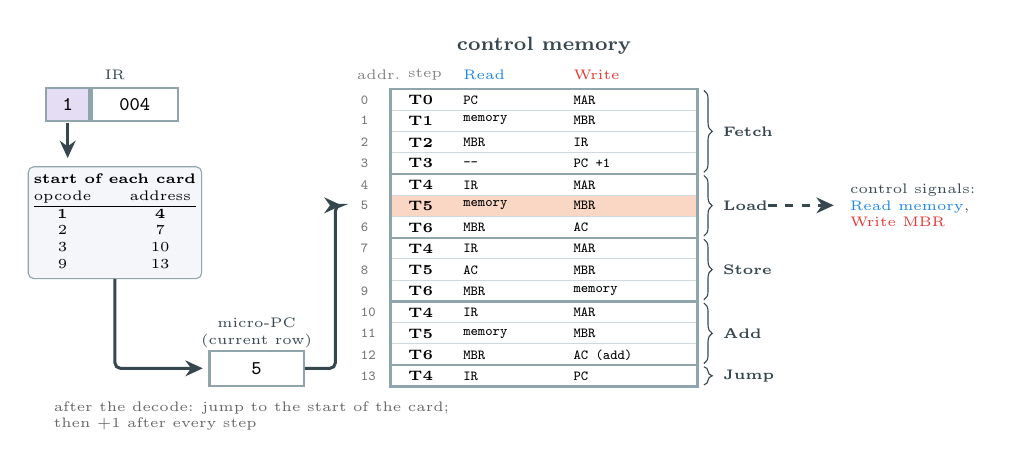
\begin{tikzpicture}[>=Stealth]
      \node[font=\scriptsize\bfseries, text=nInk] at (6.55,4.45) {control memory};
      \node[font=\tiny, text=black!50, anchor=west] at (4.05,4.08) {addr.};
      \node[font=\tiny, text=black!50, anchor=west] at (4.70,4.08) {step};
      \node[font=\tiny, text=ReadBlue, anchor=west] at (5.40,4.08) {Read};
      \node[font=\tiny, text=WriteRed, anchor=west] at (6.80,4.08) {Write};
      \draw[nLight, fill=white] (4.6,3.90) rectangle (8.5,3.63);
      \node[font=\ttfamily\tiny, text=black!55, anchor=west] at (4.10,3.76) {0};
      \node[font=\tiny\bfseries, anchor=west] at (4.70,3.76) {T0};
      \node[font=\ttfamily\tiny, anchor=west] at (5.40,3.76) {PC};
      \node[font=\ttfamily\tiny, anchor=west] at (6.80,3.76) {MAR};
      \draw[nLight, fill=white] (4.6,3.63) rectangle (8.5,3.36);
      \node[font=\ttfamily\tiny, text=black!55, anchor=west] at (4.10,3.50) {1};
      \node[font=\tiny\bfseries, anchor=west] at (4.70,3.50) {T1};
      \node[font=\ttfamily\tiny, anchor=west] at (5.40,3.50) {memory};
      \node[font=\ttfamily\tiny, anchor=west] at (6.80,3.50) {MBR};
      \draw[nLight, fill=white] (4.6,3.36) rectangle (8.5,3.09);
      \node[font=\ttfamily\tiny, text=black!55, anchor=west] at (4.10,3.22) {2};
      \node[font=\tiny\bfseries, anchor=west] at (4.70,3.22) {T2};
      \node[font=\ttfamily\tiny, anchor=west] at (5.40,3.22) {MBR};
      \node[font=\ttfamily\tiny, anchor=west] at (6.80,3.22) {IR};
      \draw[nLight, fill=white] (4.6,3.09) rectangle (8.5,2.82);
      \node[font=\ttfamily\tiny, text=black!55, anchor=west] at (4.10,2.96) {3};
      \node[font=\tiny\bfseries, anchor=west] at (4.70,2.96) {T3};
      \node[font=\ttfamily\tiny, anchor=west] at (5.40,2.96) {--};
      \node[font=\ttfamily\tiny, anchor=west] at (6.80,2.96) {PC +1};
      \draw[nLight, fill=white] (4.6,2.82) rectangle (8.5,2.55);
      \node[font=\ttfamily\tiny, text=black!55, anchor=west] at (4.10,2.68) {4};
      \node[font=\tiny\bfseries, anchor=west] at (4.70,2.68) {T4};
      \node[font=\ttfamily\tiny, anchor=west] at (5.40,2.68) {IR};
      \node[font=\ttfamily\tiny, anchor=west] at (6.80,2.68) {MAR};
      \draw[nLight, fill=AccentOrange!25] (4.6,2.55) rectangle (8.5,2.28);
      \node[font=\ttfamily\tiny, text=black!55, anchor=west] at (4.10,2.42) {5};
      \node[font=\tiny\bfseries, anchor=west] at (4.70,2.42) {T5};
      \node[font=\ttfamily\tiny, anchor=west] at (5.40,2.42) {memory};
      \node[font=\ttfamily\tiny, anchor=west] at (6.80,2.42) {MBR};
      \coordinate (hlrow) at (8.5,2.42); \coordinate (hlrowL) at (4.05,2.42);
      \draw[nLight, fill=white] (4.6,2.28) rectangle (8.5,2.01);
      \node[font=\ttfamily\tiny, text=black!55, anchor=west] at (4.10,2.14) {6};
      \node[font=\tiny\bfseries, anchor=west] at (4.70,2.14) {T6};
      \node[font=\ttfamily\tiny, anchor=west] at (5.40,2.14) {MBR};
      \node[font=\ttfamily\tiny, anchor=west] at (6.80,2.14) {AC};
      \draw[nLight, fill=white] (4.6,2.01) rectangle (8.5,1.74);
      \node[font=\ttfamily\tiny, text=black!55, anchor=west] at (4.10,1.87) {7};
      \node[font=\tiny\bfseries, anchor=west] at (4.70,1.87) {T4};
      \node[font=\ttfamily\tiny, anchor=west] at (5.40,1.87) {IR};
      \node[font=\ttfamily\tiny, anchor=west] at (6.80,1.87) {MAR};
      \draw[nLight, fill=white] (4.6,1.74) rectangle (8.5,1.47);
      \node[font=\ttfamily\tiny, text=black!55, anchor=west] at (4.10,1.60) {8};
      \node[font=\tiny\bfseries, anchor=west] at (4.70,1.60) {T5};
      \node[font=\ttfamily\tiny, anchor=west] at (5.40,1.60) {AC};
      \node[font=\ttfamily\tiny, anchor=west] at (6.80,1.60) {MBR};
      \draw[nLight, fill=white] (4.6,1.47) rectangle (8.5,1.20);
      \node[font=\ttfamily\tiny, text=black!55, anchor=west] at (4.10,1.33) {9};
      \node[font=\tiny\bfseries, anchor=west] at (4.70,1.33) {T6};
      \node[font=\ttfamily\tiny, anchor=west] at (5.40,1.33) {MBR};
      \node[font=\ttfamily\tiny, anchor=west] at (6.80,1.33) {memory};
      \draw[nLight, fill=white] (4.6,1.20) rectangle (8.5,0.93);
      \node[font=\ttfamily\tiny, text=black!55, anchor=west] at (4.10,1.06) {10};
      \node[font=\tiny\bfseries, anchor=west] at (4.70,1.06) {T4};
      \node[font=\ttfamily\tiny, anchor=west] at (5.40,1.06) {IR};
      \node[font=\ttfamily\tiny, anchor=west] at (6.80,1.06) {MAR};
      \draw[nLight, fill=white] (4.6,0.93) rectangle (8.5,0.66);
      \node[font=\ttfamily\tiny, text=black!55, anchor=west] at (4.10,0.79) {11};
      \node[font=\tiny\bfseries, anchor=west] at (4.70,0.79) {T5};
      \node[font=\ttfamily\tiny, anchor=west] at (5.40,0.79) {memory};
      \node[font=\ttfamily\tiny, anchor=west] at (6.80,0.79) {MBR};
      \draw[nLight, fill=white] (4.6,0.66) rectangle (8.5,0.39);
      \node[font=\ttfamily\tiny, text=black!55, anchor=west] at (4.10,0.52) {12};
      \node[font=\tiny\bfseries, anchor=west] at (4.70,0.52) {T6};
      \node[font=\ttfamily\tiny, anchor=west] at (5.40,0.52) {MBR};
      \node[font=\ttfamily\tiny, anchor=west] at (6.80,0.52) {AC (add)};
      \draw[nLight, fill=white] (4.6,0.39) rectangle (8.5,0.12);
      \node[font=\ttfamily\tiny, text=black!55, anchor=west] at (4.10,0.25) {13};
      \node[font=\tiny\bfseries, anchor=west] at (4.70,0.25) {T4};
      \node[font=\ttfamily\tiny, anchor=west] at (5.40,0.25) {IR};
      \node[font=\ttfamily\tiny, anchor=west] at (6.80,0.25) {PC};
      \draw[nLine, thick] (4.6,3.90) rectangle (8.5,2.82);
      \draw[decorate, decoration={brace, amplitude=3pt}, nInk] (8.58,3.88) -- (8.58,2.84);
      \node[font=\tiny\bfseries, text=nInk, anchor=west] at (8.70,3.36) {Fetch};
      \draw[nLine, thick] (4.6,2.82) rectangle (8.5,2.01);
      \draw[decorate, decoration={brace, amplitude=3pt}, nInk] (8.58,2.80) -- (8.58,2.03);
      \node[font=\tiny\bfseries, text=nInk, anchor=west] at (8.70,2.42) {Load};
      \draw[nLine, thick] (4.6,2.01) rectangle (8.5,1.20);
      \draw[decorate, decoration={brace, amplitude=3pt}, nInk] (8.58,1.99) -- (8.58,1.22);
      \node[font=\tiny\bfseries, text=nInk, anchor=west] at (8.70,1.60) {Store};
      \draw[nLine, thick] (4.6,1.20) rectangle (8.5,0.39);
      \draw[decorate, decoration={brace, amplitude=3pt}, nInk] (8.58,1.18) -- (8.58,0.41);
      \node[font=\tiny\bfseries, text=nInk, anchor=west] at (8.70,0.79) {Add};
      \draw[nLine, thick] (4.6,0.39) rectangle (8.5,0.12);
      \draw[decorate, decoration={brace, amplitude=3pt}, nInk] (8.58,0.37) -- (8.58,0.14);
      \node[font=\tiny\bfseries, text=nInk, anchor=west] at (8.70,0.25) {Jump};
      \node[draw=nLine, thick, fill=sViolet!20, minimum width=0.55cm, minimum height=0.42cm, font=\ttfamily\scriptsize] (op) at (0.5,3.7) {1};
      \node[draw=nLine, thick, fill=white, minimum width=1.1cm, minimum height=0.42cm, font=\ttfamily\scriptsize, right=0pt of op] {004};
      \node[font=\tiny, text=nInk] at (1.1,4.08) {IR};
      \node[draw=nLine, fill=LightGray, rounded corners=2pt, font=\tiny, inner sep=2pt] (map) at (1.1,2.2) {%
  \begin{tabular}{@{}cc@{}}\multicolumn{2}{@{}c@{}}{\textbf{start of each card}}\\ opcode & address\\ \hline
  \textbf{1} & \textbf{4}\\ 2 & 7\\ 3 & 10\\ 9 & 13\end{tabular}};
      \draw[line width=1.1pt, nInk, -{Stealth[length=2.2mm, width=2mm]}, shorten >= 2pt, rounded corners=2pt] (0.5,3.47) -- (0.5,2.95);
      \node[draw=nLine, thick, fill=white, minimum width=1.2cm, minimum height=0.45cm, font=\ttfamily\scriptsize] (upc) at (2.9,0.35) {5};
      \node[font=\tiny, text=nInk, align=center] at (2.9,0.8) {micro-PC\\(current row)};
      \draw[line width=1.1pt, nInk, -{Stealth[length=2.2mm, width=2mm]}, shorten >= 2pt, rounded corners=2pt] (map.south) |- (upc.west);
      \node[font=\tiny, text=black!60, align=left, anchor=north west] at (0.2,0.05) {after the decode: jump to the start of the card;\\then $+1$ after every step};
      \draw[line width=1.1pt, nInk, -{Stealth[length=2.2mm, width=2mm]}, shorten >= 2pt, rounded corners=2pt] (upc.east) -| ($(hlrowL)+(-0.15,0)$) -- (hlrowL);
      \draw[line width=1.1pt, nInk, -{Stealth[length=2.2mm, width=2mm]}, shorten >= 2pt, rounded corners=2pt, dashed] ($(hlrow)+(0.9,0)$) -- ++(0.9,0) node[right, font=\tiny, align=left] {control signals:\\\textcolor{ReadBlue}{Read memory},\\\textcolor{WriteRed}{Write MBR}};
      \end{tikzpicture}}
    \column{0.32\textwidth}
      \stepbox{Control memory}{a small memory inside the CU that holds \textbf{all the cards}.}
      \stepbox{Microinstruction}{one row: the control signals for one step.}
      \stepbox{Microprogram}{one card: the rows that carry out one machine instruction.}
      \stepbox{Micro-PC}{points to the current row, like the PC points to the current instruction.}
  \end{columns}
\end{frame}

\begin{frame}{Hardwired or microprogrammed?}
  \begin{center}
    \small
    \renewcommand{\arraystretch}{1.35}
    \begin{tabular}{lll}
      \toprule
      & \textbf{Hardwired} & \textbf{Microprogrammed} \\
      \midrule
      Speed & high & lower \\
      Design & hard when there are many instructions & simpler, systematic \\
      Changing the instructions & redesign the circuit & change the control memory \\
      Complex instructions & awkward & natural \\
      \bottomrule
    \end{tabular}
  \end{center}
  \vfill
  \keymsg{The best choice depends on how simple or complex the instructions are.}
\end{frame}

\begin{frame}{History and today}
  \begin{center}
    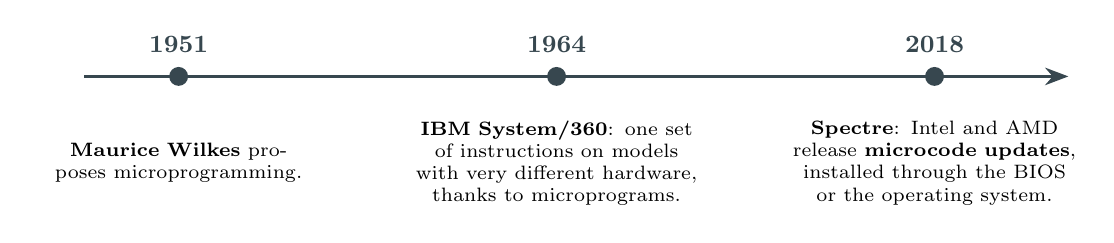
\begin{tikzpicture}[>=Stealth]
      \draw[->, very thick, nInk] (0,0) -- (12.5,0);
      \foreach \x/\y/\c in {1.2/1951/nInk, 6.0/1964/nInk, 10.8/2018/nInk} {
        \fill[\c] (\x,0) circle (0.12);
        \node[font=\small\bfseries, text=\c] at (\x,0.4) {\y};
      }
      \node[text width=3.6cm, align=center, font=\scriptsize] at (1.2,-1.1)
        {\textbf{Maurice Wilkes} proposes microprogramming.};
      \node[text width=3.6cm, align=center, font=\scriptsize] at (6.0,-1.1)
        {\textbf{IBM System/360}: one set of instructions on models with very different hardware,
         thanks to microprograms.};
      \node[text width=3.6cm, align=center, font=\scriptsize] at (10.8,-1.1)
        {\textbf{Spectre}: Intel and AMD release \textbf{microcode updates}, installed through the BIOS
         or the operating system.};
    \end{tikzpicture}
  \end{center}
  \vfill
  \keymsg{The processor in your laptop most likely contains microcode that can be updated.}
\end{frame}

% =====================================================================
\section{RISC and CISC}
% =====================================================================

\begin{frame}{From the control unit to two ideas: CISC and RISC}
  \begin{center}
    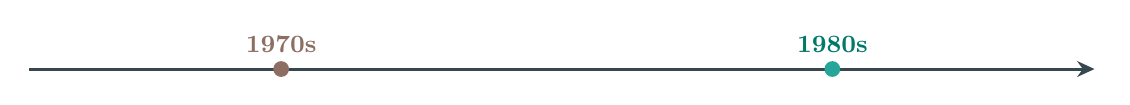
\begin{tikzpicture}[>=Stealth]
      \draw[line width=1.1pt, nInk, -{Stealth[length=2.2mm, width=2mm]}, shorten >= 2pt] (0,0) -- (13.6,0);
      \fill[sBrown] (3.2,0) circle (0.1); \node[font=\small\bfseries, text=sBrown, above] at (3.2,0.08) {1970s};
      \fill[sTeal] (10.2,0) circle (0.1); \node[font=\small\bfseries, text=sTealText, above] at (10.2,0.08) {1980s};
    \end{tikzpicture}
  \end{center}
  \vspace{-0.2cm}
  \begin{columns}[T,onlytextwidth]
    \column{0.48\textwidth}
      \begin{beamercolorbox}[rounded=true,sep=0.12cm,wd=\linewidth]{block body}
        \centering\small\textbf{More and more powerful instructions}\\[0.08cm]
        \raggedright\footnotesize
        With a \textbf{microprogrammed} CU, a new instruction is just a few new rows in the control memory.
        Memory is expensive, so short programs pay off. Designers add complex instructions,
        e.g.\ one instruction that copies a whole block of memory.
      \end{beamercolorbox}
      \vspace{0.08cm}
      \begin{beamercolorbox}[rounded=true,sep=0.1cm,wd=\linewidth]{block body example}
        \centering\footnotesize \textbf{CISC}: Complex Instruction Set Computer\\ e.g.\ VAX, x86
      \end{beamercolorbox}
    \column{0.48\textwidth}
      \begin{beamercolorbox}[rounded=true,sep=0.12cm,wd=\linewidth]{block body}
        \centering\small\textbf{Only a few simple instructions}\\[0.08cm]
        \raggedright\footnotesize
        Memory is cheaper now, and researchers (Berkeley, Stanford) notice that compilers mostly use the
        \textbf{simple} instructions. Idea: keep only simple instructions, all of the same kind,
        so a fast \textbf{hardwired} CU is enough.
      \end{beamercolorbox}
      \vspace{0.08cm}
      \begin{beamercolorbox}[rounded=true,sep=0.1cm,wd=\linewidth]{block body example}
        \centering\footnotesize \textbf{RISC}: Reduced Instruction Set Computer\\ e.g.\ MIPS, ARM, RISC-V
      \end{beamercolorbox}
  \end{columns}
  \vfill
  \keymsg{Next: what exactly is different between the two?}
\end{frame}

\begin{frame}{Two design philosophies}
  \begin{beamercolorbox}[rounded=true,sep=0.15cm,wd=\textwidth]{block body}
    \centering\large
    We will now look at \textbf{two design questions} that every processor architect must answer.
  \end{beamercolorbox}
  \vspace{0.4cm}
  
  \begin{columns}[c,onlytextwidth]
    \column{0.45\textwidth}
      \centering
      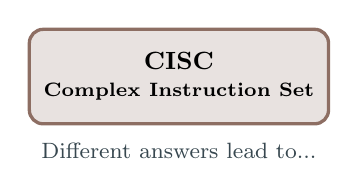
\begin{tikzpicture}[>=Stealth]
        \node[draw=sBrown, very thick, fill=sBrown!20, rounded corners=5pt, minimum width=3.8cm, minimum height=1.2cm, align=center, font=\small\bfseries] (cisc) {CISC\\[-0.05cm]\scriptsize Complex Instruction Set};
        \node[font=\footnotesize, text=nInk, anchor=north] at ([yshift=-0.1cm]cisc.south) {Different answers lead to...};
      \end{tikzpicture}
    \column{0.1\textwidth}
      \centering\Large\textbf{vs}
    \column{0.45\textwidth}
      \centering
      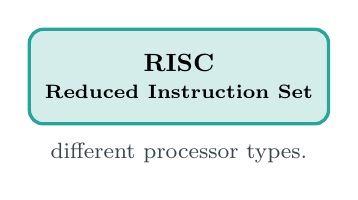
\begin{tikzpicture}[>=Stealth]
        \node[draw=sTeal, very thick, fill=sTeal!20, rounded corners=5pt, minimum width=3.8cm, minimum height=1.2cm, align=center, font=\small\bfseries] (risc) {RISC\\[-0.05cm]\scriptsize Reduced Instruction Set};
        \node[font=\footnotesize, text=nInk, anchor=north] at ([yshift=-0.1cm]risc.south) {different processor types.};
      \end{tikzpicture}
  \end{columns}
  
  \vspace{0.6cm}
  \begin{itemize}\setlength{\itemsep}{0.2cm}
    \item[\textcolor{AccentOrange}{\faArrowRight}] \textbf{Question 1:} Where can an arithmetic instruction take its values from?
    \item[\textcolor{AccentOrange}{\faArrowRight}] \textbf{Question 2:} Do all instructions have the same length?
  \end{itemize}
\end{frame}

\begin{frame}[fragile]{Question 1: where do the operands come from?}
  \centering\footnotesize The same statement \texttt{A = B + C} in three styles\\[0.1cm]
  \begin{columns}[T,onlytextwidth]
    \column{0.31\textwidth}
      \begin{beamercolorbox}[rounded=true,sep=0.1cm,wd=\linewidth]{block body}
        \centering\footnotesize\textbf{Accumulator} (MARIE)
      \end{beamercolorbox}
\begin{lstlisting}[style=marie, numbers=none]
Load  B
Add   C
Store A
\end{lstlisting}
      \scriptsize One register (AC). The ALU uses the AC and a value from memory.
    \column{0.33\textwidth}
      \begin{beamercolorbox}[rounded=true,sep=0.1cm,wd=\linewidth]{block body}
        \centering\footnotesize\textbf{Register--memory} (x86 -- CISC)
      \end{beamercolorbox}
\begin{lstlisting}[style=asm]
mov eax, [B]
add eax, [C]
mov [A], eax
\end{lstlisting}
      \scriptsize Several registers. The ALU can use a register \textbf{and} a value from memory.
    \column{0.31\textwidth}
      \begin{beamercolorbox}[rounded=true,sep=0.1cm,wd=\linewidth]{block body}
        \centering\footnotesize\textbf{Load/store} (ARM -- RISC)
      \end{beamercolorbox}
\begin{lstlisting}[style=asm]
ldr r1, B
ldr r2, C
add r3, r1, r2
str r3, A
\end{lstlisting}
      \scriptsize Many registers. The ALU uses \textbf{only registers}; only \texttt{ldr}/\texttt{str} touch memory.
  \end{columns}
  \vfill
  \keymsg{Unlike MARIE with its single AC, modern processors (both CISC and RISC) have \textbf{many registers}.}
\end{frame}

\begin{frame}{Question 2: fixed or variable instruction length?}
  \begin{center}
    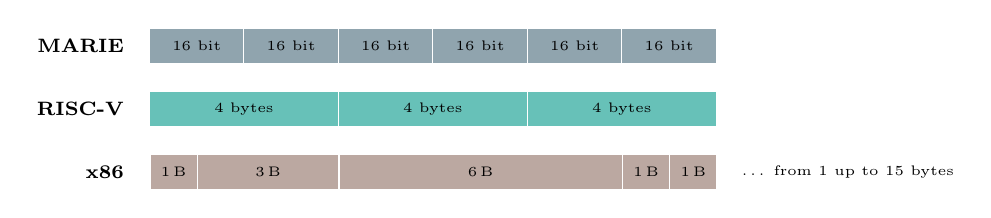
\begin{tikzpicture}
      \node[font=\scriptsize\bfseries, anchor=east] at (-0.2,0) {MARIE};
      \foreach \i in {0,...,5} \node[draw=white, fill=nLine, minimum width=1.2cm, minimum height=0.45cm,
        inner sep=0pt, font=\tiny] at ({1.2*\i+0.6},0) {16 bit};
      \node[font=\scriptsize\bfseries, anchor=east] at (-0.2,-0.8) {RISC-V};
      \foreach \i in {0,1,2} \node[draw=white, fill=sTeal!70, minimum width=2.4cm, minimum height=0.45cm,
        inner sep=0pt, font=\tiny] at ({2.4*\i+1.2},-0.8) {4 bytes};
      \node[font=\scriptsize\bfseries, anchor=east] at (-0.2,-1.6) {x86};
      \foreach \x/\w/\t in {0/0.6/1, 0.6/1.8/3, 2.4/3.6/6, 6.0/0.6/1, 6.6/0.6/1} {
        \node[draw=white, fill=sBrown!60, minimum width=\w cm, minimum height=0.45cm, inner sep=0pt,
          font=\tiny, anchor=west] at (\x,-1.6) {\t\,B};
      }
      \node[font=\tiny, anchor=west] at (7.4,-1.6) {\dots\ from 1 up to 15 bytes};
    \end{tikzpicture}
  \end{center}
  \vspace{0.25cm}
  \begin{columns}[T,onlytextwidth]
    \column{0.48\textwidth}
      \stepbox{Fixed length}{The processor knows at once where the next instruction starts,
        so fetching and decoding are simple.}
    \column{0.48\textwidth}
      \stepbox{Variable length}{Common instructions can be short, so programs take less memory.}
  \end{columns}
\end{frame}

\begin{frame}{Where does the third instruction start?}
  \begin{center}
    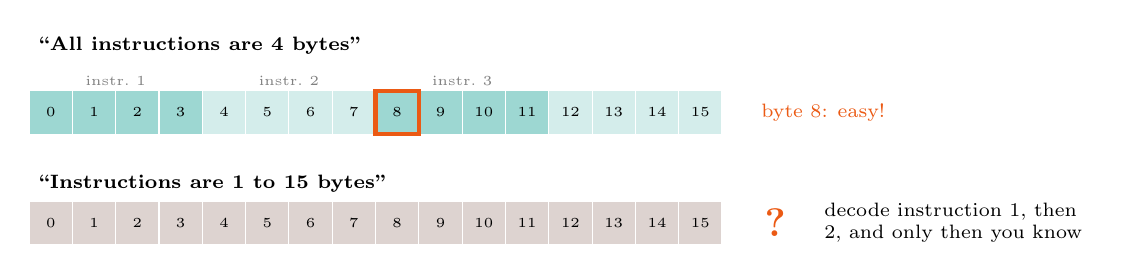
\begin{tikzpicture}
      \node[font=\scriptsize\bfseries, anchor=west] at (0,1.25) {``All instructions are 4 bytes''};
      \foreach \i in {0,...,15} {
        \pgfmathtruncatemacro{\g}{mod(floor(\i/4),2)}
        \ifnum\g=0 \def\col{sTeal!45}\else\def\col{sTeal!20}\fi
        \node[draw=white, fill=\col, minimum size=0.55cm, inner sep=0pt, font=\tiny] at ({0.55*\i+0.3},0.4) {\i};
      }
      \node[draw=AccentOrange, line width=1.5pt, minimum size=0.55cm, inner sep=0pt] at (4.7,0.4) {};
      \foreach \k/\x in {1/1.125,2/3.325,3/5.525} \node[font=\tiny, text=gray] at (\x,0.8) {instr.\ \k};
      \node[font=\scriptsize, text=AccentOrange, anchor=west] at (9.2,0.4) {byte 8: easy!};
      \node[font=\scriptsize\bfseries, anchor=west] at (0,-0.5) {``Instructions are 1 to 15 bytes''};
      \foreach \i in {0,...,15} \node[draw=white, fill=sBrown!30, minimum size=0.55cm, inner sep=0pt, font=\tiny] at ({0.55*\i+0.3},-1.0) {\i};
      \node[font=\Large\bfseries, text=AccentOrange] at (9.5,-1.0) {?};
      \node[font=\scriptsize, anchor=west, text width=3.5cm] at (10.0,-1.0) {decode instruction 1, then 2, and only then you know};
    \end{tikzpicture}
  \end{center}
  \vfill
  \keymsg{With variable length, decoding is harder. We will come back to this in a future presentation with pipelining.}
\end{frame}

\begin{frame}{RISC versus CISC}
  \begin{center}
    \small
    \renewcommand{\arraystretch}{1.2}
    \begin{tabular}{lll}
      \toprule
      & \textbf{RISC} & \textbf{CISC} \\
      \midrule
      Instructions & simple, few & complex, many \\
      Addressing modes & few & many \\
      Instruction length & fixed & variable \\
      Memory access & only load/store & also in arithmetic instructions \\
      Registers & more (32 in RISC-V) & fewer (16 in x86-64) \\
      Control unit & usually hardwired & usually microprogrammed \\
      Code size & larger: more instructions & smaller: fewer instructions \\
      Examples & ARM, RISC-V & x86 \\
      \bottomrule
    \end{tabular}
  \end{center}
  \vfill
  \begin{columns}[T,onlytextwidth]
    \column{0.48\textwidth}
      \defbox{\textbf{RISC}: Reduced Instruction Set Computer}
    \column{0.48\textwidth}
      \defbox{\textbf{CISC}: Complex Instruction Set Computer}
  \end{columns}
\end{frame}

\begin{frame}[fragile]{Exercise: CISC vs RISC execution}
  \taskhead{Individual Task}{Assume variables $X$, $Y$, and $Z$ are in memory. Write the instruction sequence for $Z=(X+Y)-2$.}
  \vspace{0.08cm}
  \begin{columns}[T,onlytextwidth]
    \column{0.48\textwidth}
      \begin{beamercolorbox}[rounded=true,sep=0.08cm,wd=\linewidth]{block body example}
        \centering\footnotesize\textbf{1. RISC style}
      \end{beamercolorbox}
      \scriptsize
      \textbf{Available instructions:}
      \begin{itemize}\setlength{\itemsep}{1.5pt}
        \item \texttt{load r, [mem]} \scalebox{0.85}{(read memory into a register)}
        \item \texttt{store r, [mem]} \scalebox{0.85}{(write a register to memory)}
        \item \texttt{add r, r1, r2} \scalebox{0.85}{(add two registers)}
        \item \texttt{sub r, r1, constant} \scalebox{0.85}{(subtract a constant)}
      \end{itemize}
    \column{0.48\textwidth}
      \begin{beamercolorbox}[rounded=true,sep=0.08cm,wd=\linewidth]{block body}
        \centering\footnotesize\textbf{2. CISC style}
      \end{beamercolorbox}
      \scriptsize
      \textbf{Additional capabilities:}
      \begin{itemize}\setlength{\itemsep}{1.5pt}
        \item \texttt{add r, [mem]} \scalebox{0.85}{(add a memory value directly)}
        \item \texttt{sub r, constant} \scalebox{0.85}{(subtract a constant from a register)}
      \end{itemize}
  \end{columns}
  \vfill
  \begin{beamercolorbox}[rounded=true,sep=0.08cm,wd=\textwidth]{block body}
    \scriptsize\raggedright
    \textbf{Compare your two solutions:}
    \begin{itemize}\setlength{\itemsep}{1pt}
      \item How many instructions did you write for RISC vs. CISC?
      \item How many times does each version access main memory?
      \item Why does the CISC version need fewer instructions?
    \end{itemize}
  \end{beamercolorbox}
\end{frame}

\begin{frame}[fragile]{Solution: CISC vs RISC execution}
  \begin{columns}[T,onlytextwidth]
    \column{0.48\textwidth}
      \begin{beamercolorbox}[rounded=true,sep=0.08cm,wd=\linewidth]{block body example}
        \centering\footnotesize\textbf{1. RISC style: 5 instructions}
      \end{beamercolorbox}
\begin{lstlisting}[style=asm]
load  r1, [X]      ; r1 = X
load  r2, [Y]      ; r2 = Y
add   r3, r1, r2   ; r3 = X + Y
sub   r3, r3, 2    ; r3 = r3 - 2
store r3, [Z]      ; Z = r3
\end{lstlisting}
    \column{0.48\textwidth}
      \begin{beamercolorbox}[rounded=true,sep=0.08cm,wd=\linewidth]{block body}
        \centering\footnotesize\textbf{2. CISC style: 4 instructions}
      \end{beamercolorbox}
\begin{lstlisting}[style=asm]
load  r1, [X]      ; r1 = X
add   r1, [Y]      ; r1 = r1 + Y
sub   r1, 2        ; r1 = r1 - 2
store r1, [Z]      ; Z = r1
\end{lstlisting}
  \end{columns}
  \vspace{0.4cm}
  \begin{columns}[T,onlytextwidth]
    \column{0.31\textwidth}
      \stepbox{Instructions}{RISC: \textbf{5}, CISC: \textbf{4}.}
    \column{0.31\textwidth}
      \stepbox{Memory accesses for data}{Both: \textbf{3}. Read $X$, read $Y$, write $Z$.}
    \column{0.31\textwidth}
      \stepbox{Why fewer in CISC?}{\texttt{add r1, [Y]} reads memory \textbf{and} adds in one instruction.}
  \end{columns}
  \vfill
  \keymsg{CISC does not save memory accesses: the load is still there, only \textbf{hidden inside} \texttt{add}.
    The work is the same, packed differently.}
\end{frame}

\begin{frame}{Today: the boundary is blurred}
  \begin{columns}[c,onlytextwidth]
    \column{0.5\textwidth}
      \centering
      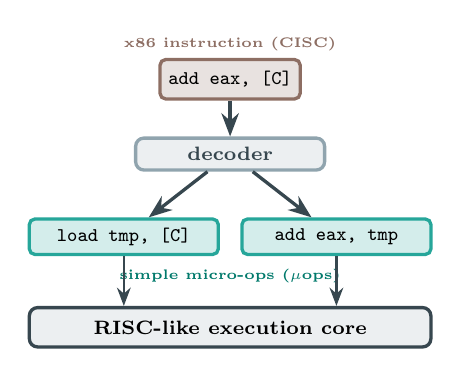
\begin{tikzpicture}[>=Stealth,
          ins/.style={draw=sBrown, very thick, fill=sBrown!20, rounded corners=2pt,
            font=\ttfamily\scriptsize, minimum height=0.5cm, inner sep=3pt},
          uop/.style={draw=sTeal, very thick, fill=sTeal!20, rounded corners=2pt,
            font=\ttfamily\scriptsize, minimum height=0.45cm, minimum width=2.4cm, inner sep=2pt}]
        \node[font=\tiny\bfseries, text=sBrown] at (0,1.55) {x86 instruction (CISC)};
        \node[ins] (x) at (0,1.1) {add eax, [C]};
        \node[draw=nLine, very thick, fill=nFill, text=nInk, rounded corners=3pt,
          font=\scriptsize\bfseries, minimum width=2.4cm] (dec) at (0,0.15) {decoder};
        \node[uop] (u1) at (-1.35,-0.9) {load tmp, [C]};
        \node[uop] (u2) at (1.35,-0.9) {add eax, tmp};
        \node[font=\tiny\bfseries, text=sTealText] at (0,-1.4) {simple micro-ops ($\mu$ops)};
        \node[draw=nInk, very thick, fill=nFill, rounded corners=3pt, font=\scriptsize\bfseries,
          minimum width=5.1cm, minimum height=0.5cm] (core) at (0,-2.05) {RISC-like execution core};
        \draw[->, very thick, nInk] (x) -- (dec);
        \draw[->, very thick, nInk] (dec) -- (u1);
        \draw[->, very thick, nInk] (dec) -- (u2);
        \draw[->, thick, nInk] (u1) -- (u1 |- core.north);
        \draw[->, thick, nInk] (u2) -- (u2 |- core.north);
      \end{tikzpicture}
    \column{0.48\textwidth}
      \stepbox{x86 (Intel, AMD)}{CISC on the outside. Since the mid-1990s (Intel Pentium Pro, 1995)
        instructions are translated \textbf{inside} into simple, RISC-like $\mu$ops.}
      \stepbox{ARM (phones, Apple M chips)}{RISC instruction set, but a very complex inside.}
      {\scriptsize\textcolor{gray}{A $\mu$op is a small RISC-like instruction. It is not the same as a MARIE micro-operation
      (one step such as \mo{MAR}{PC}), but the idea is similar: split big work into small pieces.}\par}
  \end{columns}
  \vfill
  \keymsg{RISC and CISC are \textbf{design philosophies}, not rigid categories: modern processors combine ideas from both.}
\end{frame}

\section{Summary}
% =====================================================================

\begin{frame}{What we saw today}
  \begin{center}
    
\begin{tikzpicture}[>=Stealth,
        sbox/.style={very thick, rounded corners=5pt, minimum width=2.9cm, minimum height=1.6cm,
          align=center, font=\scriptsize, text width=2.7cm, drop shadow}]
      \node[sbox, draw=nLine, fill=nFill] (a) at (0,0)
        {\textbf{Addressing modes}\\[2pt] an instruction can point to its data in different ways};
      \node[sbox, draw=nLine, fill=nFill] (b) at (3.6,0)
        {\textbf{MAR, MBR, steps}\\[2pt] every memory read costs extra steps; one bus is a bottleneck};
      \node[sbox, draw=nLine, fill=nFill] (c) at (7.2,0)
        {\textbf{Control unit}\\[2pt] sets the switches in each step: hardwired or microprogram};
      \node[sbox, draw=nLine, fill=nFill] (d) at (10.8,0)
        {\textbf{RISC and CISC}\\[2pt] two design styles, which today's processors combine};
      \draw[->, very thick, nInk] (a) -- (b);
      \draw[->, very thick, nInk] (b) -- (c);
      \draw[->, very thick, nInk] (c) -- (d);
    \end{tikzpicture}
  \end{center}
\end{frame}

\end{document}